%! TEX root = thesis.tex
% vim: ft=tex et sts=2 sw=2

\chapter[Wave localization in thin elastic structures]{Wave localization in thin elastic structures\footnote{
  This chapter is an extended version of \href{https://arxiv.org/abs/2306.07213}{M.~Mannattil and C.~D.~Santangelo, arXiv:2306.07213 [cond-mat.soft]}.
  The problem discussed in this work emerged during discussions with my coauthor.
  I was responsible for all the analytical and numerical calculations and wrote the paper taking into consideration my coauthor's comments.
}}

We consider the localization of elastic waves in thin elastic structures with spatially varying curvature profiles, using a curved rod and a singly-curved shell as concrete examples.
Previous work on related problems have largely focused on the localization of flexural waves on such structures.
Here, using the semiclassical/WKB approximation, we show that in addition to flexural waves, extensional and shear waves also form localized, bound states around points where the absolute curvature of the structure has a minimum.
These findings open up novel ways to fine-tune the acoustic and vibrational properties of thin elastic structures, and raise the possibility of introducing new phenomena not easily captured by effective models of flexural waves alone.\\[-1em]

This chapter is organized as follows.
In Section~\ref{sec:wkb}, we review the semiclassical theory of wave propagation.
We discuss wave propagation on curved rods and shells in Sections~\ref{sec:rods} and \ref{sec:shell}, respectively.
We conclude in Section~\ref{sec:conclusion}.\\[-0.5em]

\section{Introduction}
\label{sec:introduction}

Studying the propagation of elastic waves on thin structures is of crucial importance to a variety of problems in science and engineering, with applications ranging from acoustic cloaks to negative refraction~\cite{farhat2009,craster2012,zangeneh-nejad2019}.
Of particular relevance to many of these applications are localized waves, which are time-harmonic solutions to a wave equation that remain confined to a certain region of space without the presence of a confining potential or force.
Indeed, such waves are observed in many physical systems and they are often caused by heterogeneities in the medium or the boundary.
For instance, the Helmholtz equation admits bound states in arbitrary dimensions when solved on a tubular domain, provided that the tube is not everywhere straight~\cite{goldstone1992}.
Likewise, in waveguides in the form of an elastic plate, described again by coupled Helmholtz equations, waves localize around points of maximal curvature~\cite{gridin2005}.
Bound waves of similar nature have also been predicted in waveguides in the form of rods~\cite{gridin2005a}, elastic strips with varying elastic moduli~\cite{forster2006} and thickness~\cite{postnova2008}, quantum waveguides~\cite{duclos1995}, etc.

Localized waves can also arise in elastodynamic systems described by higher-order wave equations.
In this context, \citet{scott1992} studied the localized vibrations of a musical saw---an ordinary hand saw bent into the shape of the letter \textsf{S} and playable like a musical instrument~\cite{leonard1989,stuckenbruck2016}.
More recently, \citet{shankar2022} revisited the musical saw using both experiments and theory.
Forgoing an explicit analytical computation of the mode frequencies, they argued that the bound modes that appear at the inflection point of the saw are topologically protected.
Localization of elastic waves on variably-curved shells, such as the musical saw, is not entirely surprising as it is known that curvature acts as an effective refractive index for such waves~\cite{norris1994,evans2013}.

Motivated by the above studies, in this paper, we investigate further aspects of curvature-controlled localization of waves in thin elastic structures, choosing a singly-curved shell and a curved rod as our examples.
If the structure is uncurved, there are three basic types of waves that can propagate.
Extensional waves propagate by stretching and compressing the structure, and involve only the tangential displacements ($u$ and $v$ in Fig.~\ref{fig:waves}).
Flexural waves, by contrast, propagate by bending the structure and involve only the normal displacement ($\zeta$ in Fig.~\ref{fig:waves}).
In flat plates, shear waves, which do not compress or expand the plate, and involving only the tangential displacements propagate as well~\cite{landau1986}.

The situation gets complicated when the structure is curved.
First, curvature tends to couple the tangential and normal displacements, and therefore, we can only speak of waves that are predominantly flexural or extensional or shear like.
Second, there are no universally accepted elastodynamic equations for curved structures, and in case of the rod and the shell, several choices exist~\cite{morley1961,pierce1993,doyle2021,kernes2021}.
The simplest ones, however, are almost always a set of linear partial differential equations that couple the normal and tangential displacements, the independent variables being time and the coordinates that describe the undeformed configuration of structure ($x$ and $y$ in Fig.~\ref{fig:waves}).
The physical assumptions usually made (expressed here in terms of the wave number $k$ and the structure's curvature $m$) while writing down such a set of equations are~\cite{pierce1993,norris1994,kernes2021}:
%
\begin{enumerate}
  \item The wavelength ($\sim k^{-1}$) is much larger that the thickness of the structure.
    If we work in length units such that the thickness is of order unity, we must then have $k \ll 1$.
    For bulk waves with wavelengths much smaller than the thickness (i.e., when $k \gg 1$), the structure should be treated as an infinite elastic medium~\cite{landau1986}.
  \item The radius of curvature is much larger than the thickness, so that $\abs{m} \ll 1$ (in length units such that thickness is order unity).
  \item The wavelength is smaller or of the order magnitude as the radius of curvature ($= m^{-1}$), so that $k > m$ is a safe choice (in all length units).
\end{enumerate}

Because the curvature couples the different displacement components, irrespective of the equations we use, to fully characterize wave propagation on curved structures, we have to consider multicomponent (i.e., vector) waves.
Computing the exact spectrum of a multicomponent differential operator is often difficult, unless one resorts to numerical techniques.
Indeed, for this reason, in their theoretical analyses of the musical saw, both \citet{scott1992}, and \citet{shankar2022} chose to simplify matters by analyzing flexural vibrations alone.
%
\begin{figure}
  \begin{center}
    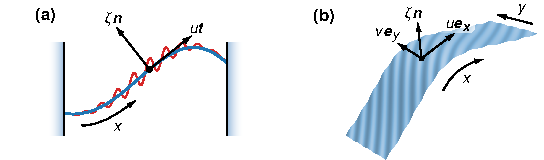
\includegraphics{localization/waves.pdf}
  \end{center}
  \caption{
    Waves can propagate on thin elastic structures such as (a) rods and (b) shells.
    The undeformed structure is parameterized by the coordinates $x$ and $y$.
    Curvature couples tangential displacements ($u$ and $v$) that stretch/shear the structure with normal displacements ($\zeta$) that bend it.
  }
  \label{fig:waves}
\end{figure}

As we have remarked \hl{previously}, the semiclassical/WKB approximation is a widely used technique to obtain asymptotic solutions to wave problems, including those describing the elastodynamics of thin structures~\cite{pierce1970,nielsen2014,sndergaard2016,mohammed2021}.
Additionally, in wave equations supporting bound-state solutions, the semiclassical approximation allows one to extract the corresponding frequencies through quantization.
In multicomponent equations, however, subtleties can arise owing to the presence of an extra phase in the quantization rule~\cite{yabana1986,kaufman1987,littlejohn1991,littlejohn1991a}.
Recently, this phase has been shown~\cite{venaille2023} to be responsible for a spectral flow in the rotating shallow-water equations that describe oceanic waves on the Earth's surface, leading to the topological protection of equatorial waves~\cite{delplace2017}.

In this paper, we use the semiclassical approximation to study the bound-state spectrum of elastic waves in a curved rod and a singly-curved shell with a varying curvature profile.
To avoid losing the main results of the paper in a thicket of details, we summarize them here:
%
\begin{enumerate}
  \setlength\itemsep{0em}
  \item[(i)] For both the rod and the shell, independent of the boundary conditions, waves exhibit robust localization around points where the absolute curvature has a minimum.
    Wave localization induced by the presence of an inflection point in an $\mathsf{S}$-shaped musical saw~\cite{scott1992,shankar2022} is a special case of this more general observation.
    These findings also complement the prediction by \citet{mohammed2021} regarding the localization of flexural waves in a curved shell around points of maximal curvature.
  \item[(ii)] In a curved rod, only extensional waves form bound states and flexural waves always form ``unbound'' states that are spread across the rod.
  \item[(iii)] In a shell, waves of all three types can form states that are bound along the curved direction
    [$x$ in Fig.~\ref{fig:waves}(b)].
    In the frequency spectrum, flexural bound states appear first and have the lowest frequencies.
    They are then followed by shear and extensional bound states, in that order.
  \item[(iv)] For both structures, flexural waves start propagating well below the frequency of the first bound state associated with an extensional wave.
    Hence, in very long rods and shells, these bound states coexist with a near-continuum of flexural waves, forming quasi bound states in a continuum~\cite{hsu2016}.
  \item[(v)]
    Finally, both structures are described by equations for which the extra phase in the modified quantization rule vanish---something that we expect to be generically true for equations of thin-walled structures.
    This simplifies our analysis considerably and results in remarkable agreement between the quantization results and numerical experiments.
\end{enumerate}

Our findings show that waves can be robustly trapped in thin elastic structures by a simple alteration of their geometry.
This could help, for instance, in crafting better thin-plate acoustic cloaks~\cite{farhat2009}, and aid the control of noise and vibration in thin structures~\cite{mace1987,hansen2012}.
Curvature-induced localization of waves could also be used to improve the acoustic black-hole effect in thin-walled structures~\cite{lee2017,pelat2020}, which at the moment relies primarily on wave localization caused by a power-law tapered thickness profile~\cite{krylov2020}.
Finally, a singly-curved shell serves as a simple, yet effective single-mode waveguide that can steer flexural waves of specific frequencies in the uncurved direction.

\section{Semiclassical theory of waves}
\label{sec:wkb}

In this section we present a quick rundown of the semiclassical approximation as applied to multicomponent waves.
For more detailed descriptions, we refer to the book by \citet{tracy2014}.
Consider a wave equation of the form
%
\begin{equation}
  \partial_{t}^{2}\Psi(x,t) + \widehat{\mathsf{H}}\Psi(x,t) = 0,
  \label{eq:full_wave_eq}
\end{equation}
%
where $\Psi(x,t)$ is an $N$-component wave field described by a one-dimensional coordinate $x$ and time $t$.
In elastodynamics, $\Psi$ is usually composed of displacements, e.g., for the rod we have $\Psi = (\zeta, u)$, and for the shell we have $\Psi = (\zeta, u, v)$ [see Figs.~\ref{fig:waves}(a) and~\ref{fig:waves}(b)].
Also, $\widehat{\mathsf{H}}$ is taken to be a Hermitian operator in the form of an $N\times N$ matrix, composed solely of spatial derivatives (i.e., powers of $\partial_{x}$) with time-independent coefficients.
Assuming that the waves are time harmonic with frequency $\omega$, i.e., $\Psi(x, t) = \psi(x)e^{\pm i\omega t}$, where $\psi(x)$ is the time-independent part of the wave field, Eq.~\eqref{eq:full_wave_eq} can be recast as
%
\begin{equation}
  \widehat{\mathsf{D}}\psi = 0,\quad \text{with}\enspace \widehat{\mathsf{D}} = \widehat{\mathsf{H}} - \omega^{2}\mathsf{I}_{N},
  \label{eq:ev_problem}
\end{equation}
%
where $\mathsf{I}_{N}$ is the $N\times N$ identity matrix.
If the coefficients of the spatial derivatives that appear in $\widehat{\mathsf{D}}$ are constants, then the eigenmodes $\psi$ are plain waves.
In what follows we assume that these coefficients are slowly varying, with the variation controlled by a single positive parameter $\epsilon \ll 1$.
It is useful to treat $\epsilon$ as an ordering parameter so that we can look for solutions at various orders of $\epsilon$.
To this end, we rescale $x \to \epsilon^{-1}x$ so that a derivative $\partial_{x}$ becomes $\epsilon \partial x$.
With analogy to quantum mechanics, this allows us to recast the derivatives in $\widehat{\mathsf{D}}$ in terms of the wave number/momentum operator $\hat{k} = -i\epsilon \partial_{x}$, with $\epsilon$ playing the role of Planck's constant.
Since we shall be considering $\widehat{\mathsf{D}}$ in the coordinate representation, the position operator $\hat{x} = x$.

We look for \emph{eikonal} solutions to Eq.~\eqref{eq:ev_problem} of the form $\psi(x) = A(x)e^{iS(x)/\epsilon}$, where the amplitude $A(x)$ is an $N$-component spinor with complex components, and $S(x)$ is a rapidly varying phase, playing the role of an action.
In order to solve Eq.~\eqref{eq:ev_problem} at various orders of $\epsilon$, it is convenient to make use of Weyl calculus, which allows one to map differential operators that are functions of $\hat{x}$ and $\hat{k}$ to ordinary functions, called Weyl symbols, defined on an $x$-$k$ phase space, and vice versa~\cite{chaichian2001,cohen2012}.
For the purposes of this paper, the following simple rules suffice to convert operators to symbols:
%
\begin{equation}
  f(x) \to f(x),\enspace
  g(\hat{k}) \to g(k),\enspace\text{and}\enspace
  f(x)g(\hat{k}) \to f(x)g(k) + \frac{i\epsilon}{2}f'(x)g'(k) + \mathcal{O}(\epsilon^{2}).
  \label{eq:weylrules}
\end{equation}
%
Above, $f$ and $g$ are functions of $x$ and $\hat{k}$, with the primes denoting derivatives.

Converting each entry of the matrix operator $\widehat{\mathsf{D}}$ into a Weyl symbol, we get the $N\times N$ dispersion matrix $\mathsf{D}$, which we express in various orders of $\epsilon$ as $\mathsf{D} = \mathsf{D}^{(0)} + \epsilon\mathsf{D}^{(1)} + \mathcal{O}(\epsilon^{2})$.
Employing the eikonal ansatz, at $\mathcal{O}(\epsilon^{0})$, we find the matrix equation $\mathsf{D}^{(0)}A = 0$.
To satisfy this equation, at least one of the $N$ eigenvalues of $\mathsf{D}^{(0)}$, say $\lambda(x, k;\, \omega)$, must vanish so that $\det \mathsf{D}^{(0)}(x, k; \omega) = 0$.
A vanishing eigenvalue $\lambda$ and the associated normalized eigenvector $\tau$ describes different wave types or ``polarizations'' represented by Eq.~\eqref{eq:ev_problem}.
By a polarization we mean a linear subspace of the total wave field that is usually of a distinct physical nature, e.g., flexural waves on a curved rod.
Semiclassical approximation breaks down near points where more than one eigenvalues of $\mathsf{D}^{(0)}$ simultaneously vanish, precipitating an exchange of energy and mode conversion between waves of different polarizations~\cite{tracy2014}.

In the absence of mode conversion, the vanishing eigenvalues of $\mathsf{D}^{(0)}$ also serve as the \emph{ray Hamiltonian} of waves of a specific polarization.
 This leads us to the phase-space representation of waves as rays that satisfy the Hamilton's equations
%
\begin{equation}
  \dot{x} = \partial_{k} \lambda(x, k;\, \omega) = \left\{x, \lambda\right\}
  \quad\text{and}\quad
  \dot{k} = -\partial_{x} \lambda(x, k;\, \omega) = \left\{k, \lambda\right\},
\end{equation}
%
where the overdot denotes derivatives with respect to a parameter that parameterizes the rays and $\left\{\cdot, \cdot\right\}$ is the $x$-$k$ Poisson bracket.
Since the waves we consider propagate in a one-dimensional space, these rays are identical to the level curve defined by $\lambda(x, k; \omega) = 0$.
%
\begin{figure}
  \begin{center}
    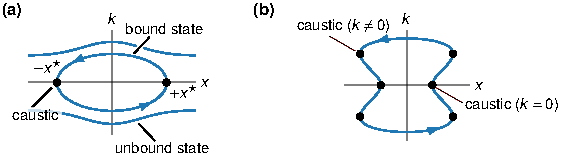
\includegraphics{localization/caustic.pdf}
  \end{center}
  \caption{%
    (a) In phase space, bound states are represented by rays in the form of closed orbits, which is analogous to that of a bound particle oscillating between two classical turning points ($\pm x^{\star}$ in the cartoon).
    Other trajectories represent unbound states.
    (b) A bound state represented by a ``peanut''-shaped orbit has six caustics.%
  }
  \label{fig:caustic}
\end{figure}

\subsection{Bound waves in phase space}

We expect the rays of bound waves to be bounded in phase space as well, with these rays being topologically equivalent to a circle~\cite{keller1958,mcdonald1988}.
Such rays oscillate between two classical turning points where $k = 0$ and $\dot{x} = 0$ [Fig.~\ref{fig:caustic}(a)].
Turning points are examples of caustics, i.e., points on the ray where $\dot{x} = 0$, and in a bound ray, apart from the classical turning points, there could be other caustics as well [see Fig.~\ref{fig:caustic}(b)].
Even though the semiclassical approximation breaks down near the caustics, we can recover the phase $S(x)$ by integrating $k(x)$ along a ray.
Furthermore, for bound rays, single valuedness of $\psi(x)$ results in the modified Bohr--Sommerfeld quantization condition
%
\begin{equation}
  \epsilon^{-1}\oint \dd{x}\,k(x;\, \omega) = 2\left(n + \frac{\alpha}{4}\right)\pi - \gamma,
  \label{eq:quantization}
\end{equation}
%
from which bound-state frequencies can be obtained.
Above, the quantum number $n \in \mathbb{N}_{0}$ and $\alpha$ is the Keller--Maslov index~\cite{keller1958,maslov1981}.
Closed orbits in a two-dimensional phase space that can be smoothly deformed to a small circle always have $\alpha = 2$~\cite{percival1977}.
The additional phase $\gamma$ only appears when the wave field has more than one component, and is a consequence of the fact that the polarization vector $\tau$ is uniquely determined only up to an overall phase.
Its rate of change $\dot{\gamma}$ as we move along a ray can be written as $\dot{\gamma} = \dot{\gamma}_{\text{G}} + \dot{\gamma}_{\text{NG}}$, with~\cite{yabana1986,kaufman1987,venaille2023}
%
\begin{equation}
\dot{\gamma}_{\text{G}} = i\tau_{j}^{*}\left\{\tau_{j}, \lambda\right\} %= i{\tau_{j}}^{*}\dot{\tau}_{j}
  \quad\text{and}\quad
  \dot{\gamma}_{\text{NG}} = \frac{i}{2}\mathsf{D}^{(0)}_{jk}\left\{\tau^{*}_{j}, \tau_{k}\right\} - \tau_{j}^{*}\mathsf{D}^{(1)}_{jk}\tau_{k},
\label{eq:extra_phases}
\end{equation}
%
where the asterisk represents complex conjugation and the subscripts $j, k$ represent the entries and components of $\mathsf{D}^{(0)}$ and $\tau$, respectively.
It can be shown that the first phase $\gamma_{\text{G}}$ has the general form of a geometric phase~\cite{pancharatnam1956,berry1984} upon treating the $x$-$k$ phase space as a parameter space~\cite{yabana1986}.
The second (non-geometric) phase $\gamma_{\text{NG}}$ has no such interpretation.

%%
%\begin{equation}
%\gamma_{\text{G}} = \oint \dd{\sigma}\, \dot{\gamma}_{\text{G}} = i\oint \dd{\sigma}\,\left\langle{\tau_{\alpha}}\middle|\dot{\tau}_{\alpha}\right\rangle =
%  i\oint \dd\xi\cdot\left\langle{\tau_{\alpha}}\middle|\nabla_{\xi}\tau_{\alpha}\right\rangle,
%\end{equation}
%%
%where $\xi = (x, k)$ denotes the ``parameters'' that are being varied.

%In Appendix~\ref{app:additional_phase} we prove that $\gamma_{\text{G}}$ vanishes if the relative phases between the components of the eigenvector $\tau_{\alpha}$ are constants.
%The second (non-geometric) phase $\gamma_{\text{NG}}$ need not vanish in such a situation, however.
Instead of explicitly accounting for the extra phase $\gamma$ in the quantization rule, we could have diagonalized the wave equation at various orders of $\epsilon$~\cite{littlejohn1991,littlejohn1991a,weigert1993,venaille2023}.
During such a procedure, terms proportional to $\dot{\gamma}_{\text{G}}$ and $\dot{\gamma}_{\text{NG}}$ naturally appear in the ray Hamiltonian $\lambda$ as a first-order correction.
Despite the elegance of the method, we do not use it in our analysis.
This is because, as we discuss in Appendix~\ref{app:additional_phase}, for both the problems we consider, the extra phases vanish.

\section{Waves on a curved rod}
\label{sec:rods}

As we remarked earlier, several rod theories~\cite{chidamparam1993,walsh2000}, with varying levels of sophistication, have been written down for describing wave propagation on rods---straight or curved.
For our purposes, a simple linear model~\cite{kernes2021} of a curved rod would do.
This model ignores higher-order effects like torsion, cross-sectional rotation, etc., and can be viewed as the lower-dimensional analogue of the Donnell--Yu shell model~\cite{donnell1933,yu1955} that we shall later use to understand wave propagation on curved shells.

\subsection{Equations of motion and semiclassical approximation}
\label{sec:rod_equations}

Let the undeformed state of the rod be in the form of a plane curve $\bm{\sigma}: \mathcal{X} \to \mathbb{R}^{2}$, which we take to be parameterized by its arclength $x \in \mathcal{X} \subset \mathbb{R}$.
As a wave propagates along the rod, it undergoes a deformation $\bm{\sigma} \to \bm{\sigma} + \delta\bm{\sigma}$, where the displacement field $\delta\bm{\sigma}(x,t) = u(x,t)\bm{t}(x) + \zeta(x,t)\bm{n}(x)$.
Here $\bm{t} = \dd\bm{\sigma}/\dd{x}$ is the unit tangent of the undeformed rod and $\bm{n}$ is its unit normal, obtained by rotating $\bm{t}$ counter-clockwise by $\pi/2$ [see Fig.~\ref{fig:waves}(a)].
Using $\zeta$ and $u$ as the components of the wave field, and assuming the absence of external forces, the rod equations we are after is derived from the following energy functional~\cite{kernes2021}:
%
\begin{equation}
  \mathscr{U}[\zeta, u] = \int \dd{t}\,\dd{x}\,\frac{1}{2}\left\{\rho\left(\dot{u}^{2} + \dot{\zeta}^{2}\right) - E\left[\partial_{x}u - m(x)\zeta\right]^{2} - B\left(\partial_{x}^{2}\zeta\right)^{2}\right\}.
  \label{eq:rod_energy}
\end{equation}
%
Above, we have assumed that the rod is uniform with linear mass density $\rho$, with extensional stiffness $E$ and bending stiffness $B$.
Also, the signed curvature of the rod is $m(x) = \bm{n}\cdot\dd\bm{t}/\dd{x}$, which we assume to vary with the arclength $x$.
With these identifications, we can delineate the bending and stretching contributions to the energy.%
\footnote{%
  The stretching contribution to the energy is approximated by taking the usual one-dimensional strain $\partial_{x}u$ and adding to it the circumferential strain, which for a (convex) differential element of the rod with angular width $\delta\theta$ and radius $r = -m^{-1}$ is roughly $[(r + \zeta)\delta{\theta} - r\delta\theta]/(r\delta\theta) = -m\zeta$~\cite{donnell1933}.
The bending energy, on the other hand, is the usual Euler--Bernoulli bending energy, without any additional curvature-dependent corrections.
See Section~\ref{sec:rod_ho} for a rod model that includes additional corrections to the bending energy.}
Upon varying the energy functional~$\mathscr{U}$, we get the dynamic rod equations
%
\begin{subequations}
\begin{align}
  \label{eq:rod_flex}
  \rho\partial_{t}^{2}\zeta &= -B\partial_{x}^{4}\zeta - Em(x)\left[m(x)\zeta - \partial_{x}u\right],\\
  \rho\partial_{t}^{2}u &= -E\left\{\partial_{x}\left[m(x)\zeta\right] - \partial_{x}^{2}u\right\}.
  \label{eq:rod_ext}
\end{align}
\end{subequations}
%
When the curvature $m = 0$, Eq.~\eqref{eq:rod_flex} reduces to the dynamic Euler--Bernoulli equation representing purely transverse flexural waves that propagate by bending the rod.
In the same limit, Eq.~\eqref{eq:rod_ext} characterizes extensional waves that propagate longitudinally by stretching the rod.
When curvature is nonzero, which is the case we want to analyze, the components $\zeta$ and $u$ remain coupled.

In terms of the rod's Young's modulus $Y$, cross-sectional area $A$, and its second moment of area $I$, the extensional and bending stiffnesses are $E = YA$ and $B = YI$, respectively.
If the rod's cross-sectional ``thickness'' is $h$, then $A \sim h^2$ and $I \sim h^{4}$.
This gives a natural length unit $\ell = \sqrt{B/E} \sim h$ and a time unit $\sqrt{B\rho}/E$ that can be used to conveniently nondimensionalize the rod equations.
Noting that under a change of length units the curvature transforms as $m(x) \to \ell^{-1}m(x)$, we arrive at the nondimensional form of the rod equations, which in matrix form reads [cf. Eq.~\eqref{eq:full_wave_eq}]
%
\begin{equation}
\partial_{t}^{2}
\begin{pmatrix}
  \zeta\\
  u
\end{pmatrix} +
\widehat{\mathsf{H}}
\begin{pmatrix}
  \zeta\\
  u
\end{pmatrix} = 0,
\enspace
\text{where}
\enspace
\widehat{\mathsf{H}}
=
\begin{pmatrix}
  \partial^{4}_{x} + m^{2}(x) & -m(x)\partial_{x}\\
  m(x)\partial_{x} + m'(x) & -\partial^{2}_{x}
\end{pmatrix}.
\label{eq:rod}
\end{equation}
%
Although this is a rather simple set of coupled equations involving the curvature $m(x)$ as the only parameter, a nonuniform $m(x)$ makes obtaining a general solution difficult.

To employ the semiclassical approximation for solving Eq.~\eqref{eq:rod}, we assume that the curvature is a slowly varying function of the form $m(\epsilon x)$.
Here $0 < \epsilon \ll 1$ is a small dimensionless parameter that controls the slowness of the variation.
Because the length unit $\ell$ we chose for nondimensionalizing the arclength $x$ is proportional to the thickness, physically speaking, here we are assuming that the length scale over which the curvature varies significantly is much larger that the thickness of the rod.
%(The actual length scale over which the curvature varies significantly is $\epsilon^{-1}\ell$.)
Next, we do a final change of variables $x \to \epsilon^{-1}x$ in Eq.~\eqref{eq:rod} so that $m(\epsilon x) \to m(x)$ and all spatial derivatives get multiplied by $\epsilon$.
For the eigenvalue problem with $\widehat{\mathsf{D}} = \widehat{\mathsf{H}} - \omega^{2}\mathsf{I}_{2}$, this gives us
%
\begin{equation}
 \widehat{\mathsf{D}} =
 \begin{pmatrix}
    \epsilon^{4}\partial^{4}_{x} + m^{2}(x) - \omega^{2} & -m(x)\epsilon\partial_{x}\\
    m(x)\epsilon\partial_{x} + \epsilon m'(x) & -\epsilon^{2}\partial^{2}_{x} - \omega^{2}
 \end{pmatrix}
=
 \begin{pmatrix}
   \hat{k}^{4} + m^{2}(x) -\omega^{2} & -i m(x)\hat{k}\\
    im(x)\hat{k} + \epsilon m'(x) & \hat{k}^{2} - \omega^{2}
\end{pmatrix}.
\label{eq:filwaveop}
\end{equation}
%
In the final step above, we have set $\epsilon\partial_{x} \to i\hat{k}$, with $\hat{k}$ being the momentum operator.
Using the rules in Eq.~\eqref{eq:weylrules} we can easily write down the Weyl symbol $\mathsf{D}$ for the operator in Eq.~\eqref{eq:filwaveop} as
$\mathsf{D} = \mathsf{D}^{(0)} + \epsilon\mathsf{D}^{(1)}$, where
%
\begin{equation}
\mathsf{D}^{(0)} =
 \begin{pmatrix}
    {k}^{4} + m^{2}(x) - \omega^{2} & -i m(x){k}\\
    im(x){k} & {k}^{2} - \omega^{2}
\end{pmatrix}
\enspace \text{and} \enspace
\mathsf{D}^{(1)} =
\frac{1}{2}
\begin{pmatrix}
    0 & m'(x)\\
    m'(x) & 0
\end{pmatrix}.
\label{eq:rod_D}
\end{equation}

The two eigenvalues of the dispersion matrix $\mathsf{D}^{(0)}$, representing waves of two different polarizations, are
%
\begin{equation}
  \lambda_{\pm} = \frac{1}{2}\left\{k^{2} + k^{4} + m^{2}(x) \pm \sqrt{\left[k^{2} - k^{4} - m^{2}(x)\right]^{2} + 4k^{2}m^{2}(x)}\right\} - \omega^{2}.
  \label{eq:rod_ham}
\end{equation}
%
For a given $\omega$, we have $\lambda_{+}(x, k;\, \omega) \geq \lambda_{-}(x, k;\, \omega)$ for all values of $x$ and $k$.
Mode conversion between the two polarizations ensues near points where $\lambda_{+}(x, k;\, \omega) = \lambda_{-}(x, k;\, \omega)$, and the semiclassical approximation breaks down.
But from Eq.~\eqref{eq:rod_ham}, we see that $\lambda_{+} = \lambda_{-}$ only when the discriminant in Eq.~\eqref{eq:rod_ham} vanishes, which happens only when $m(x)$ is zero, and $k = \pm 1$ or $k = 0$.
As we discussed in Section~\ref{sec:introduction}, the rod equations are only applicable for short waves whose wavelength is much longer than the thickness, which translates to the requirement $0 \ll \abs{k} \ll 1$.
Hence, mode-conversion points with $k = \pm 1$ or $k = 0$, lie well beyond the range of applicability of these equations.
For this reason, we ignore mode-conversion issues and assume that $\lambda_{+} \neq \lambda_{-}$ throughout our analysis.
Before moving on, it is useful to first analyze the propagation of waves on a rod of constant curvature.

\subsection{Rods of constant curvature}

First we analyze the case where the curvature is zero, i.e., when the rod is straight.
In the limit of vanishing curvature $m$, we should recover the dispersion relations $\omega(k)$ for plane waves propagating on a straight rod from $\lambda_{\pm}$.
On setting $m = 0$ and noting that $\abs{k} \ll 1$, we see that $\lambda_{+} = 0$ gives us the linear dispersion relation $\omega = k$, representing extensional waves propagating on a straight rod.
Meanwhile, when $m = 0$, we find that $\lambda_{-} = 0$ gives us the quadratic dispersion relation $\omega = k^{2}$ of flexural waves on a straight rod.
%For this reason, from now on we shall call waves represented by $\lambda_{-}$ as flexurally polarized waves and those represent by $\lambda_{+}$ as extensionally polarized waves.

For nonzero, but constant curvature, the rod forms part of a ring.
If the curvature is sufficiently weak, we expect the eigenvalue $\lambda_{+}$ to continue to represent predominantly extensional waves and $\lambda_{-}$ to represent predominantly flexural waves.
To verify this, we expand $\lambda_{\pm}$ in powers of $m^{2}$ and drop powers of $k$ in comparison to unity to find
%
\begin{equation}
  \lambda_{+} = k^{2} + m^{2} - \omega^{2} + \mathcal{O}(m^{4})
  \quad\text{and}\quad
  \lambda_{-} = k^{4} - k^{2}m^{2} - \omega^{2} + \mathcal{O}(m^{4})
  \qquad{(k \gg m)}.
  \label{eq:rod_kgm}
\end{equation}
%
Clearly, the above expansions can only be valid when the $\mathcal{O}(m^{2})$ correction terms are less than the lowest-order terms, which is true only when $k \gg m$.
In this limit we have $\lambda_{+} \sim k^{2} - \omega^{2}$ and $\lambda_{-} \sim k^{4} - \omega^{2}$, confirming our expectation.

We next look at the case where both $k$ and $m$ are small,%
\footnote{%
  We consider this limit to analyze the behavior of the waves close to a classical turning point where $k = 0$.
  The wave decays beyond a turning point and it never gets a chance to complete a full-wavelength oscillation with $k \ll m$, so that the short wavelength assumption is not violated.
}
but with $k \ll m$.
To this end, we expand $\lambda_{\pm}$ in powers of $km^{-1}$ to find
%
\begin{equation}
  \lambda_{+} = k^{2} + m^{2} - \omega^{2} + \mathcal{O}(k^{4})
  \quad\text{and}\quad
  \lambda_{-} = \frac{k^{6}}{m^{2}}\left[1 + \mathcal{O}\left(\frac{k^{2}}{m^{2}}\right)\right] - \omega^{2}
  \qquad{(k \ll m)}.
  \label{eq:rod_klm}
\end{equation}
%
Dispersion relations obtained from setting $\lambda_{\pm} = 0$ above show significant deviation from those of a straight rod and we expect the waves of both polarizations to result in bending and stretching of the rod.
For the same reason, we expect both these waves to have both longitudinal and transverse characteristics.
Despite this, for the sake of simplicity and identification, we shall continue to call waves represented by $\lambda_{+}$ as extensional waves and those represented by $\lambda_{-}$ as flexural waves.

Bending of the rod is associated with normal component $\zeta$ and stretching with tangential component $u$.
To better understand how the two components contribute to the wave field in the presence of curvature, we define the amplitude ratio
%
\begin{equation}
  \mathscr{R} = \frac{\abs{\zeta}}{\abs{\zeta} + \abs{u}}.
  \label{eq:rod_ratio}
\end{equation}
%
With the above definition, for purely transverse and longitudinal waves $\mathscr{R} = 1$ and $\mathscr{R} = 0$, respectively.
In the eikonal ansatz, at the lowest order, the wave field $\psi = (\zeta, u)$ is proportional to the eigenvectors $\tau_{\pm}$ of $\mathsf{D}^{(0)}$ so that $\zeta \sim \tau_{\pm,1}$ and $u \sim \tau_{\pm,2}$.
Making use of Eqs.~\eqref{eq:rod_kgm} and \eqref{eq:rod_klm}, to the lowest order in $k$ and $m$, the eigenvectors $\tau_{\pm}$ are
%
\begin{equation}
  \tau_{+} \sim \left(m,\enspace ik\right)
  \quad\text{and}\quad
  \tau_{-} \sim \left(ik,\enspace m\right),
  \label{eq:rod_tau}
\end{equation}
%
so that the asymptotic amplitude ratios for the two wave polarizations become $\mathscr{R}_{+} \sim \abs{m}/(\abs{m} + \abs{k})$ and $\mathscr{R}_{-} \sim \abs{k}/(\abs{m} + \abs{k})$.
For $m = 0$, we know that extensional waves become entirely longitudinal, and as expected the corresponding amplitude ratio $\mathscr{R}_{+} = 0$.
In same limit, flexural waves become entirely transverse as indicated by $\mathscr{R}_{-} = 1$.
However, for small values of $k$ with $k \ll m$ we see that $\mathscr{R}_{+} \to 1$ and $\mathscr{R}_{-} \to 0$.
In other words, in the limit $k \ll m$, waves of the two polarizations would switch their nature from being predominantly longitudinal to being predominantly transverse, and vice versa.

\subsection{Rods with varying curvature}

For illustrative purposes, we consider rods of two curvature profiles $m_{1}(x)$ and $m_{2}(x)$, defined~by
%
\begin{equation}
  m_{1}(x) = b\tanh(\epsilon x)
  \quad\text{and}\quad
  m_{2}(x) = b - \left(b - a\right)\sech(\epsilon x),
  \label{eq:rod_curv}
\end{equation}
%
which we will informally call tanh- and sech-type curvature profiles, respectively.
Above, $b$ and $a$ are positive constants such that $a < b$ and the parameter $\epsilon$ controls the slowness of variation of the curvatures.
A rod with a tanh-type curvature profile $m_{1}(x)$ possesses an inflection point at $x=0$ where the curvature vanishes, and the curvature asymptotes to $\pm b$ as $x\to \pm\infty$ [see Figs.~\ref{fig:rod_bound}(a) and~\ref{fig:rod_bound}(b)].
On the other hand, a rod with a sech-type curvature profile $m_{2}(x)$ remains concave for all $x$, with the curvature acquiring its minimum value of $a$ at $x = 0$ and asymptoting to $b$ as $x\to\pm\infty$ [see Figs.~\ref{fig:rod_bound}(c) and~\ref{fig:rod_bound}(d)].
For the purpose of illustrating our results, we take $b = 0.1$ and $a = 0.01$, so that the smallest ratio between the radius of curvature and thickness is $\mathcal{O}(10)$.
Although such a ratio is comparatively smaller than typical experimental values, it would give us a clearer picture of the effects of a varying curvature profile.
We also set $\epsilon = 0.01$, but as we rescale $x \to \epsilon^{-1}x$, the parameter $\epsilon$ does not always explicitly appear in our discussions.
Note also that the numerical values of the local wave number $k$ is unaffected by this rescaling.

For a varying curvature profile, we find the rays for both polarizations by integrating the corresponding Hamilton's equations given by
%
\begin{equation}
  \begin{alignedat}{2}
      \dot{x} &= \frac{\partial \lambda_{\pm}}{\partial k} &&= k\left\{2k^{2} + 1 \pm \frac{(2k^{2} + 1)\left[k^{2} + k^{4} + m^{2}(x)\right] - 6k^{4}}{\sqrt{\left[k^{2}-k^{4}-m^{2}(x)\right]^{2} + 4k^{2}m^{2}(x)}}\right\};\\
      \dot{k} &= -\frac{\partial \lambda_{\pm}}{\partial x} &&= -\frac{1}{2}\left[m^{2}(x)\right]'\left\{1 \pm \frac{k^{2} + k^{4} + m^{2}(x)}{\sqrt{\left[k^{2}-k^{4}-m^{2}(x)\right]^{2} + 4k^{2}m^{2}(x)}}\right\}.
  \end{alignedat}
  \label{eq:rod_hamiltonian}
\end{equation}
%
\begin{figure}
  \begin{center}
    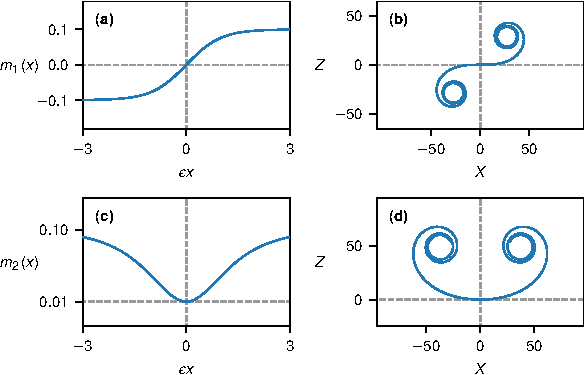
\includegraphics{localization/rod_profile.pdf}
  \end{center}
  \caption{%
    (a) Tanh-type curvature profile $m_{1}(x)$ with an inflection point at $x = 0$ and (b) the corresponding shape of the rod in Cartesian space with coordinates $X$ and $Z$.
    (c) Sech-type curvature profile $m_{2}(x)$ with no inflection point and (d) the corresponding shape of the rod.
    For both curvature types, as the arclength $x \to \pm\infty$, the rod becomes part of a circle.
    In all figures $a = 0.01$, $b = 0.1$, and $\epsilon = 0.01$.
  }
  \label{fig:rod_profile}
\end{figure}

\subsection{Extensional waves}
\label{sec:extensional}

We first discuss how a varying curvature profile affects extensional waves in a rod.
In Section~\ref{sec:extensional_limit} we present an alternative approach, where we analyze the extensional limit of the rod equations and show that extensional waves form bound states.
The purpose here, however, is to understand this using a semiclassical perspective, which will serve as a basis for understanding the variably-curved shell.

As we discussed previously, extensional waves are to be associated with the ray Hamiltonian $\lambda_{+}$.
Without loss of generality, let $x = 0$ be a point where $m^{2}(x)$ has a local extremum, so that its derivative $[m^{2}(x)]'\big|_{x=0} = 0$ and the origin $(0, 0)$ becomes a fixed point of the Hamilton's equation in Eq.~\eqref{eq:rod_hamiltonian} for $\lambda_{+}$.
Since Eq.~\eqref{eq:rod_hamiltonian} is a Hamiltonian system, the origin becomes a nonlinear center or a saddle depending on whether the Hamiltonian $\lambda_{+}(x, k)$, viewed as a function of $x$ and $k$, has an extremum or a saddle there~\cite{strogatz1994,jordan2007}.
For the present problem, we find two situations%
\footnote{We can also infer this from the sign of the Hessian determinant of $\lambda_{+}$ at $(0, 0)$ given by $\det \nabla\nabla \lambda_{+}\big|_{x=0,k=0} = 2(m^{2})''\big|_{x=0}$, provided that $(m^{2})'' \neq 0$ so that the origin is a nondegenerate fixed point with $\det\nabla\nabla\lambda_{+} \neq 0$.}
depending on the behavior of $m^{2}(x)$ at $x = 0$.
%
\begin{enumerate}
    \item[(i)]
  \emph{$m^{2}$ has a nonzero maximum at $x = 0$.\enspace}
  Then, for any point $x$ sufficiently close to $0$, we have $m^{2}(x) < m^{2}(0) = \lambda_{+}(0, 0)$.
  We also see that $\lambda_{+}(x, 0) - \lambda_{+}(0, 0) < 0$, whereas $\lambda_{+}(0, k) - \lambda_{+}(0, 0) > 0$.
  In other words, if we move along the $x$ axis from the origin $(0, 0)$, the value of $\lambda_{+}(x, k)$ decreases, whereas moving along the $k$ axis increases its value, showing that the origin becomes a saddle point.

  \item[(ii)] \emph{$m^{2}$ has a minimum at $x = 0$.\enspace}
    At any point $(x, k)$ sufficiently close to $(0, 0)$, we have $m^{2}(x) > m^{2}(0)$.
    Then, using basic inequality arguments, $\lambda_{+}(x, k) - \lambda_{+}(0, 0) > 0$, showing that $\lambda_{+}$ has a minimum at the origin, which means that it becomes a nonlinear center.
\end{enumerate}
%
As the extrema of $m^{2}(x)$ are identical to the extrema of the absolute curvature $\abs{m(x)}$, we can summarize as follows: points where the absolute curvature has a minimum become nonlinear centers of the ray equations associated with $\lambda_{+}$, and points where the absolute curvature has a maximum become saddles.
Therefore, we expect extensional waves to get trapped only around points where the absolute curvature has a minimum.
%
\begin{figure}
  \begin{center}
    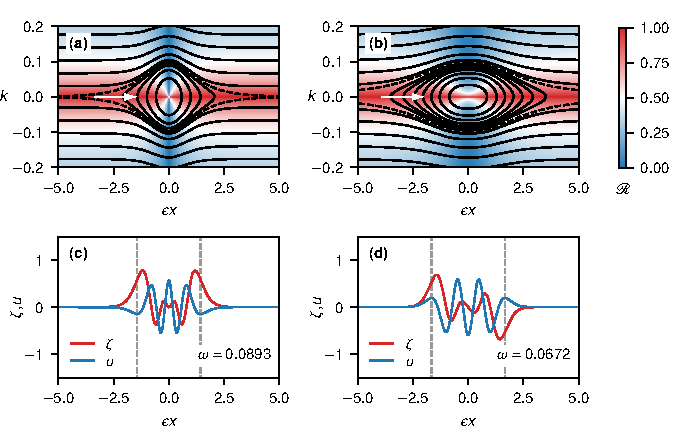
\includegraphics{localization/rod_bound.pdf}
  \end{center}
  \caption{%
    Ray trajectories for extensional waves on a rod with (a) tanh-type curvature profile $m_{1}(x)$ and (b) sech-type curvature profile $m_{2}(x)$, with the phase portraits color coded using the amplitude ratio $\mathscr{R}$ defined in Eq.~\eqref{eq:rod_ratio}.
    The white arrows in (a) and (b) indicate rays of the same frequency as the two bound states in (c) and (d).
    The grey vertical lines in (c) and (d) indicate the locations of the classical turning points.
  }
  \label{fig:rod_bound}
\end{figure}

The black curves in Figs.~\ref{fig:rod_bound}(a) and~\ref{fig:rod_bound}(b) show the extensional rays for the two curvature profiles.
Each ray is a level curve defined by $\lambda_{+}(x, k; \omega) = 0$ for a specific $\omega$.
Since $\lambda_{+}$ is invariant with respect to reflection about the $x$ and $k$ axes, the ray trajectories also share the same reflection symmetry.
For both curvature types, there are three fixed points: the origin $(0, 0)$ and $(\pm\infty, 0)$.
The fixed points at $(\pm\infty, 0)$ are saddles since $m^{2}(x)$ achieves its maximum there.
Two heteroclinic orbits, shown as black dashed curves, connect the fixed points at $(\pm\infty, 0)$.
% The origin is always a nondegenerate fixed point for a tanh-type curvature profile since $[m_{1}^{2}(x)]''\big|_{x=0} = 2b^{2}$.
% For the sech-type curvature profile, the origin is a nondegenerate fixed point only when $a$ is nonzero so that $[m_{2}^{2}(x)]''\big|_{x=0} = 2a(b - a) > 0$.
As per our analysis, the origin is always a center as $m^{2}(x)$ achieves a minimum there for both curvature types.
Close to the origin, the rays appear in form of closed orbits indicating bound states.

Before we present some example results, it is useful to analyze the parity of the bound states.
If $\psi(x) = \left[\zeta(x), u(x)\right]$ is a bound state, then it is easy to check that for an odd curvature profile $m(x)$ with $m(-x) = m(x)$, the eigenmode $\psi(-x) = \left[\zeta(-x), u(-x)\right]$ is also a bound state satisfying the rod equations, Eq.~\eqref{eq:rod}, with the boundary conditions $\psi(\pm\infty) = 0$.
Assuming nondegeneracy in the eigenmodes, we must then have $\left[\zeta(x), u(x)\right] = \pm\left[\zeta(-x), u(-x)\right]$, which means that for an odd $m(x)$, the components $\zeta(x)$ and $u(x)$ must have the same parity, i.e., they are either both odd or both even.%
\footnote{%
  More quantum mechanically, this can be shown by considering the commutation of $\widehat{\mathsf{D}}$ with the operators $\widehat{\mathsf{P}}_{\pm} = \diag\left(\widehat{\pi}, \pm\widehat{\pi}\right)$, where $\widehat{\pi}$ is the usual parity operator~\cite{cohen-tannoudji2019}.
  Clearly, $\widehat{\mathsf{P}}_{\pm}\Psi(x) = \left[\zeta(-x), \pm u(-x)\right]$ so that
  the eigenstates of $\widehat{\mathsf{P}}_{+}$ always have $\zeta(x)$ and $u(x)$ of the same parity, whereas the eigenstates of $\widehat{\mathsf{P}}_{-}$ always have $\zeta(x)$ and $u(x)$ of different parity.
  Furthermore, for odd and even $m(x)$, we can show that $\widehat{\mathsf{D}}$ commutes with $\widehat{\mathsf{P}}_{+}$ and $\widehat{\mathsf{P}}_{-}$, respectively.
  As commuting operators share the same eigenstates (assuming nondegeneracy), this proves the claim made above.%
}
For an even $m(x)$, however, we find that bound-state solutions must satisfy $\left[\zeta(x), u(x)\right] = \pm\left[\zeta(-x), -u(-x)\right]$, showing that the components $\zeta(x)$ and $u(x)$ always have different parity.
In Figs.~\ref{fig:rod_bound}(c) and~\ref{fig:rod_bound}(d) we show two example bound states obtained by solving the rod equations numerically (see Appendix \ref{app:numerical} for details) and depicting both components of the wave field $\psi$.
Consistent with our analysis, the example bound state of the tanh-type curvature profile has even $\zeta(x)$ and $u(x)$.
Likewise, for the example bound state of the sech-type curvature profile, $\zeta(x)$ is odd and $u(x)$ is even.

Clearly, the displacement fields of the bound states of both curvature profiles show a significant presence of both normal and tangential components.
To understand this better, consider again the phase portraits in Fig.~\ref{fig:rod_bound}(a) and \ref{fig:rod_bound}(b), which have been color coded using the amplitude ratio $\mathscr{R}$ defined in Eq.~\eqref{eq:rod_ratio}, and computed%
\footnote{Note that we are using the exact expression for $\tau_{+}$ and not the approximate expression in Eq.~\eqref{eq:rod_tau} to find $\mathscr{R}$.  Using the approximate expression would also result in nearly similar results.}
from the components of the polarization vector $\tau_{+}$.
The closed orbits corresponding to the example bound states have been marked with white arrows in these phase portraits.
Starting at the $k$ axis, if we move along a closed orbit towards one of its turning points, we see that $\mathscr{R}$ changes from $0$ to $1$, indicating that the wave acquires a strong normal component, which is what we see from the example bound states.

The existence of the bound states can also be intuitively understood from the dispersion relations for extensional waves.
From Eq.~\eqref{eq:rod_ham}, we see that at $k = 0$, the dispersion curve given by $\lambda_{+} = 0$ has a nonzero gap and a cut-on frequency%
\footnote{Incidentally, this cut-on frequency is the ring frequency of extensional waves, i.e., when the wavelength is equal to the circumference of a ring of radius $m^{-1}$~\cite{walsh2000}.}
of $\omega_{\text{cut-on}}^{2} = m^{2}$.
For waves with $\omega < \omega_{\text{cut-on}}$, the wave number $k$ is always complex, preventing the wave from being able to propagate and the wave decays.
Now, as an extensional wave enters a region of high curvature from a region of low curvature, the local cut-on frequency increases.
This means that, at some point, the frequency of the wave would fall below the local cut-on frequency, and the wave gets reflected creating a bound state.
As the cut-on frequency depends only on the magnitude of the curvature, and not its sign, bound states do not require the presence of an inflection point---an observation that was also made by \citet{scott1992} while analyzing the musical saw.
%
\begin{figure}
  \begin{center}
    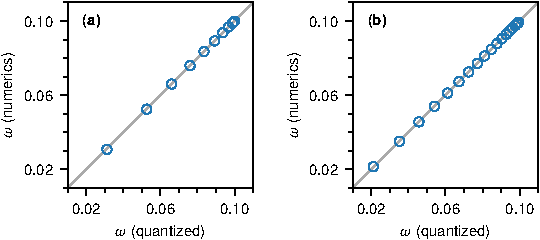
\includegraphics{localization/rod_wkb.pdf}
  \end{center}
  \caption{
    Bound-state frequencies obtained from numerics compared to that obtained through quantization for a rod with (a) tanh-type curvature profile and (b) sech-type curvature profile.
    In both plots, the gray guide line in the background represents $\omega$ (numerics) = $\omega$ (quantized).
  }
  \label{fig:rod_wkb}
\end{figure}

\subsubsection*{Quantization and bound states}

In order to evaluate the action in the quantization condition, Eq.~\eqref{eq:quantization}, in principle, we should express $k$ in terms of $x$ from $\lambda_{+}(x, k; \omega) = 0$.
This proves to be difficult as $k$ would then have to be obtained as the root of a sixth-order polynomial.
Instead, as described in Appendix~\ref{app:numerical}, we compute the action by numerically integrating $k(x)$ between the classical turning points $\pm x^{\star}$.
Setting $k = 0$ in $\lambda_{+}(x, k; \omega) = 0$, we see that these points are implicitly given by the equation $m^{2}(x^{\star}) = \omega^{2}$.
To quantize the bound orbits, we also need the Keller--Maslov index, which is $\alpha = 2$ as the orbits are topologically equivalent to a circle.
Now, note that the off-diagonal operators of the matrix $\widehat{\mathsf{D}}$ in the rod equations, Eq.~\eqref{eq:rod}, are composed only of odd derivatives.
In Appendix~\ref{app:additional_phase}, we show that the additional phase $\gamma$ in Eq.~\eqref{eq:quantization}, vanishes for any operator of this form, enabling us to find the quantized frequencies without additional difficulty.
A comparison between the numerically obtained bound-state frequencies and those obtained through quantization (Fig.~\ref{fig:rod_wkb}) shows excellent agreement between the two.
Furthermore, these frequencies are independent of the boundary conditions chosen to solve the rod equations, showing the robustness of the bound states.

Instead of computing the action by quadrature, we could have extracted $k(x)$ from the approximate expression for $\lambda_{+}$ [see Eqs.~\eqref{eq:rod_kgm} and \eqref{eq:rod_klm}], which gives $k(x) \approx \pm\sqrt{\omega^{2} - m(x)^{2}}$.
This expression can be used, for instance, to estimate the maximum number of bound states $n_{\text{max}}$ for the two curvature profiles.
The largest frequency for which we see an extensional bound state is $\omega = b$.
As shown in Figs.~\ref{fig:rod_bound}(a) and~\ref{fig:rod_bound}(b), the rays corresponding to this frequency form two heteroclinic orbits connecting the classical turning points at $x = \pm \infty$.
Computing the area inside these orbits, we find
%
\begin{equation}
  n_{\text{max}} \approx \frac{1}{\pi\epsilon}\int_{-\infty}^{+\infty} \dd{x}\,k(x) =
  \begin{dcases}
    b/\epsilon & \text{(tanh type)},\\
    \bar{b}/\epsilon + \mathcal{O}(a/\epsilon) & \text{(sech type)}.
  \end{dcases}
  \label{eq:rod_maxb}
\end{equation}
%
Here, $\bar{b} = \pi^{-1}b\int_{-\infty}^{\infty}\dd{x}\,\sech{x}\sqrt{2\cosh{x} - 1} \approx 2b$.
Therefore, we expect an infinitely long rod with a sech-type curvature profile to support twice as many bound states as a rod with a tanh-type curvature profile.
A similar expression for $n_\text{max}$ is also derived in Appendix~\ref{sec:extensional_limit} where we directly consider the extensional limit of the rod equations, and find the quantized frequencies as well as the bound modes.

For the values $b = 0.1$ and $\epsilon = 0.01$ we use in our examples, Eq.~\eqref{eq:rod_maxb} predicts a maximum of 10 bound states for a tanh-type rod and 20 bound states for a sech-type rod.
This prediction is consistent with our numerical experiments with a finite-sized rod, where we find a total of 10 and 18 bound states for the two curvature profiles.
Despite this, we only expect a small number of extensional bound states in actual experiments with curved rods, where we expect the finiteness of the rod to become more important.
For one thing, as the arc length $x \to \pm\infty$, self intersection is inevitable for both sech- and tanh-type rods having a nonzero thickness (see Fig.~\ref{fig:rod_profile}).
(Self-intersection effects, however, can be ameliorated if we allow for small motions of the rod perpendicular to the plane containing it.)
Furthermore, as the turning points of the higher-frequency bound states are far apart, they do not always appear to be spatially localized, even though they decay exponentially as $x \to \pm\infty$.
%
\begin{figure}
  \begin{center}
    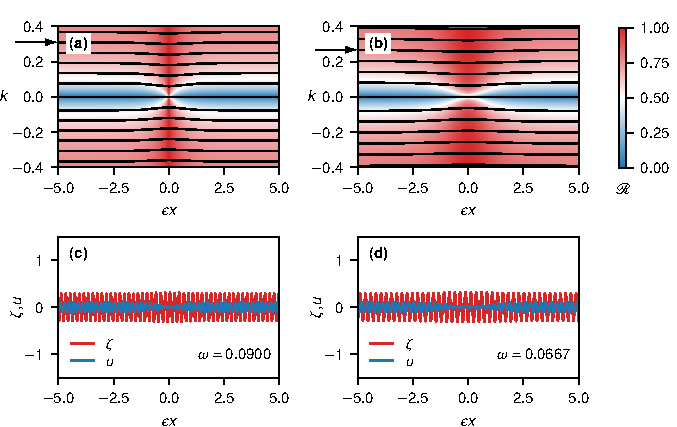
\includegraphics{localization/rod_extended.pdf}
  \end{center}
  \caption{%
    Ray trajectories for flexural waves on a rod with (a) tanh-type curvature profile $m_{1}(x)$ and (b) sech-type curvature profile $m_{2}(x)$, with the phase portraits color coded using the ratio $\mathscr{R}$ defined in Eq.~\eqref{eq:rod_ratio}.
    The black arrows in (a) and (b) indicate rays of the same frequency as the two eigenmodes in figures (c) and (d).
  }
  \label{fig:rod_extended}
\end{figure}

\subsection{Flexural waves}

Flexural waves are associated with the ray Hamiltonian $\lambda_{-}$ and from the corresponding Hamilton's equations in Eq.~\eqref{eq:rod_hamiltonian}, we see that the derivatives $\dot{x}$ and $\dot{k}$ vanish everywhere on the $x$ axis.
Since there are no isolated fixed points anywhere on the $x$ axis for these rays, we do not expect flexural waves to form bound states.
This is confirmed by the phase portraits in Figs.~\ref{fig:rod_extended}(a) and~\ref{fig:rod_extended}(b).
Like rays of extensional waves, the rays of flexural waves are also invariant under reflection about the $x$ and $k$ axes because $\lambda_{-}$ possesses the same symmetry.
Two unbound flexural eigenmodes obtained numerically are displayed in Figs.~\ref{fig:rod_extended}(c) and~\ref{fig:rod_extended}(d).
Rays corresponding to these modes have been marked by black arrows in Figs.~\ref{fig:rod_extended}(a) and~\ref{fig:rod_extended}(b).
Although the normal component $\zeta$ dominates in these modes, they acquire a significant tangential component with increasing curvature, which we also see from the color coding of the phase portraits.

Although the frequencies of the extensional bound states in Figs.~\ref{fig:rod_bound}(c) and~\ref{fig:rod_bound}(d) and the flexural eigenmodes in \ref{fig:rod_extended}(c) and~\ref{fig:rod_extended}(d) are rather close, the mode profiles differ significantly in appearance.
Also, the frequencies of the flexural eigenmodes depend on the specific boundary conditions chosen and other physical parameters, e.g., the total length of the rod.
When the rod length increases, we expect flexural waves to form a near continuum in the frequency spectrum, whereas the frequencies of the extensional bound states would continue to be determined by the quantization condition, Eq.~\eqref{eq:quantization}.
Setting $\lambda_{-} = 0$ and putting $k = 0$ in Eq.~\eqref{eq:rod_ham}, we also see that flexural waves in a rod are gapless and start propagating well below the first bound extensional state.
In this sense, in very long rods, extensional bound states appear as quasi-bound states in a continuum of flexural waves.

\section{Extensional limit of the rod equations}
\label{sec:extensional_limit}

We define the extensional limit of the rod equations as the limit in which the average bending energy of a deformed rod is considerably smaller than its stretching energy.
The bending energy in the rod model we use is proportional to $(\partial_{x}^{2} \zeta)^{2}$ [see Eq.~\eqref{eq:rod_energy}], which gives rise to the fourth-order derivative $\partial_x^{4}\zeta$ in the rod equations, Eq.~\eqref{eq:rod}.
Neglecting this term and Fourier transforming in time, we find the extensional limit of the rod equations, which take the form
%
\begin{subequations}
  \begin{align}
  \label{eq:rod_ext1}
  m(x)\left[m(x)\zeta(x) - \partial_{x}u(x)\right] &= \omega^{2}\zeta(x),\\
  \partial_{x}\left[m(x)\zeta(x) - \partial_{x}u(x)\right] &= \omega^{2}u(x).
  \label{eq:rod_ext2}
  \end{align}
\end{subequations}
%
The above equations possess a soft-mode solution with $\omega = 0$ satisfying $m(x)\zeta(x) = \partial_{x}u(x)$, which corresponds to all linear isometries that do not stretch the rod to the lowest order.
%
\begin{figure}
  \begin{center}
    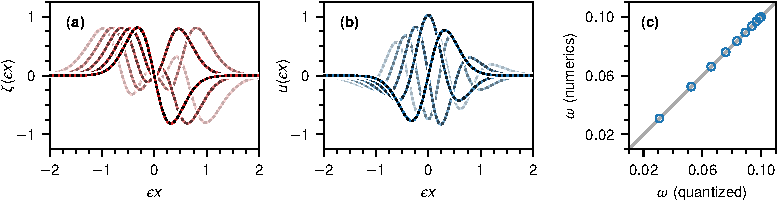
\includegraphics{localization/rod_poschl.pdf}
  \end{center}
  \caption{%
    The first five extensional bound states of a rod with a tanh-type curvature profile showing (a) the normal component $\zeta(x)$ and (b) the tangential component $u(x)$, with lighter curves depicting higher-frequency states.
    The dashed black curves in (a) and (b) represent the solutions in Eq.~\eqref{eq:poschl}.
    (c) Comparison between the bound-state frequencies $\omega$ obtained through quantization, and those from numerics [cf.~Fig.~\ref{fig:rod_wkb}(a)].
  }
  \label{fig:poschl}
\end{figure}

We now look for bound-state solutions of Eqs.~\eqref{eq:rod_ext1} and \eqref{eq:rod_ext2} satisfying $\zeta(\pm\infty) = u(\pm\infty) = 0$ with vanishing derivatives at $x = \pm\infty$.
Let us additionally assume that the longitudinal component $u(x) = \partial_{x}\phi(x)$, where $\phi(x)$ is an unknown differentiable function satisfying%
\footnote{Assuming $\phi(\pm\infty) = 0$ does not result in any loss in generality.
Without this assumption, on integrating Eq.~\eqref{eq:rod_ext2} we see that $\phi(\pm\infty) = C$ (constant).
We then obtain Eq.~\eqref{eq:schrodinger} in terms of $\widetilde{\phi}(x) = \phi(x) - C$ with $\zeta = m\widetilde{\phi}$, so that we can work in terms of $\widetilde{\phi}$ alone, which is equivalent to setting $C = 0$.}
$\phi(\pm\infty) = 0$.
Equation~\eqref{eq:rod_ext2} then becomes a total derivative, which on integration yields
%
\begin{equation}
  m(x)\zeta(x) = \partial_{x}^{2}\phi(x) + \omega^{2}\phi(x).
\end{equation}
%
Putting the above equation in Eq.~\eqref{eq:rod_ext1} and ignoring the soft-mode solution with $\omega = 0$, we see that $\zeta(x) = m(x)\phi(x)$, from which we deduce that $\phi(x)$ satisfies a Schr\"{o}dinger-like equation with the potential $m^{2}(x)$, and given by
%
\begin{equation}
  -\partial_{x}^{2}\phi(x) + m^{2}(x)\phi(x) = \omega^{2}\phi(x).
  \label{eq:schrodinger}
\end{equation}
%
As is well known from elementary quantum mechanics~\cite{buell1995}, Eq.~\eqref{eq:schrodinger} always admits a bound-state solution provided that potential $m^{2}(x)$ has a minimum.

For the tanh-type curvature profile with $m = m_{1}(x) = b\tanh(\epsilon x)$, Eq.~\eqref{eq:schrodinger} becomes the time-independent Schr\"{o}dinger equation for a particle in a P\"{o}schl--Teller potential~\cite{poschl1933,rosen1932}, whose solutions $\phi(x)$ can be written in terms of the associated Legendre polynomials $P^{\mu}_{\nu}(\,\cdot\,)$~\cite{olver2010}.
On defining
%
\begin{equation}
  \kappa(x) = \tanh(\epsilon x),
  \quad
  \nu = \frac{1}{2}\left[\sqrt{1 + 4b^{2}/\epsilon^{2}} - 1\right],
  \quad\text{and}\quad
  \mu = n - \nu \leq 0
  \quad(n \in \mathbb{N}_{0}),
  \label{eq:poschl_params}
\end{equation}
%
and solving for $\phi(x)$, we find the (unnormalized) components $\zeta(x) = m(x)\phi(x)$, $u(x) = \partial_{x}\phi(x)$, and the quantized frequencies to be
%
\begin{equation}
  \zeta(x) = b\kappa(x)P^{\mu}_{\nu}\left[\kappa(x)\right],
  \quad
  u(x) = \partial_{x}P^{\mu}_{\nu}\left[\kappa(x)\right],
  \quad\text{and}\quad
  \omega^{2} = b^{2} - \epsilon^{2}\mu^{2}.
  \label{eq:poschl}
\end{equation}
%
Figure~\ref{fig:poschl} presents a comparison of the bound states described by Eq.~\eqref{eq:poschl} and the numerical results for extensional bound states.
The agreement is remarkable given the fact that the numerical results were obtained by solving the full wave equations, Eq.~\eqref{eq:rod}, without employing any additional approximations.
From Eq.~\eqref{eq:poschl_params} we also see that maximum number of bound states is $n_{\text{max}} \approx \nu = b/\epsilon + \mathcal{O}(b^{2}/\epsilon^{2})$, which agrees with the semiclassical prediction in Eq.~\eqref{eq:rod_maxb}.

We are currently unaware of an exact solution of Eq.~\eqref{eq:schrodinger} for the potential $\smash{m^{2}_{2}(x)\allowbreak = \left[b - (b - a)\sech(\epsilon x)\right]^{2}}$ corresponding to a sech-type curvature profile, even though exact solutions for similar potentials exist~\cite{lemieux1969,nieto1978,ishkhanyan2018}.
However, we can crudely approximate $m^{2}_{2}(x)$ as a deformed P\"{o}schl--Teller potential of the form
%
\begin{equation}
  m^{2}_{\chi}(x) = b^{2} - (b^{2} - a^{2})\sech^{2}(\epsilon\chi x).
\end{equation}
%
We fix the deformation parameter $\chi$ by demanding that the full widths at half minima of both $m^{2}_{\chi}(x)$ and $m_{2}^{2}(x)$ be equal, which gives
%
\begin{equation}
  \chi = \sech^{-1}\sqrt{\frac{b^{2} + a^{2}}{2(b^{2} - a^{2})}}\Bigg/\sech^{-1}\left[\frac{b - \sqrt{(b^{2} - a^{2})/2}}{b - a}\right].
\end{equation}
%
When $b = 0.1$, $a=0.01$, the deformation parameter $\chi \approx 0.49$ and $m_{\chi}(x)$ approximates $m(x)$ to around 97\% accuracy when $\abs{x} > \frac{1}{2}\Delta$, where $\Delta$ is the full width at half maximum.
The approximation becomes significantly worse for $\abs{x} < \frac{1}{2}\Delta$, with a maximum relative error of 68\%.
Therefore, we only expect the higher-frequency bound states of $m_{\chi}(x)$ to represent states of $m(x)$ reasonably well, which is exactly what we see from the results in Fig.~\ref{fig:poschl_sech}.
%
\begin{figure}
  \begin{center}
    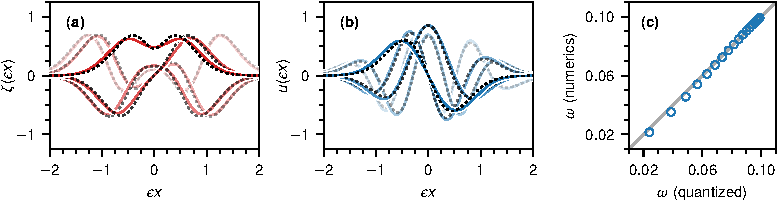
\includegraphics{localization/rod_poschl_sech.pdf}
  \end{center}
  \caption{%
    The first five extensional bound states of a rod with a sech-type curvature profile showing (a) the normal component $\zeta(x)$ and (b) the tangential component $u(x)$.
    Lighter curves in (a) and (b) depict higher-frequency states and the dashed black curves represent the solutions obtained analogously to those in Eq.~\eqref{eq:poschl} after setting $b^{2} \to b^{2} - a^{2}$ and $\epsilon \to \chi\epsilon$.
    (c) Comparison between the bound-state frequencies $\omega$ obtained through quantization, and those from numerics [cf.~Fig.~\ref{fig:rod_wkb}(b)].
  }
  \label{fig:poschl_sech}
\end{figure}

At this juncture, let us remark that Eq.~\eqref{eq:schrodinger} can also be derived by diagonalizing the full wave equation in Eq.~\eqref{eq:rod} using the asymptotic method outlined by Littlejohn and coworkers~\cite{littlejohn1991,littlejohn1991a,weigert1993}, without appealing to any physical arguments.
In this method, the operators of the diagonalized equations in symbol form are the two eigenvalues $\lambda_{\pm}$ of the dispersion matrix $\mathsf{D}^{(0)}$.
To find the extensional bound states, we focus on $\lambda_{+}$, the ray Hamiltonian for extensional waves.
Instead of using $\lambda_{+}$ from Eq.~\eqref{eq:rod_ham}, which involves a radical expression, we use the approximate version $\lambda_{+} \approx k^{2} - m^{2} - \omega^{2}$ [see Eqs.~\eqref{eq:rod_kgm} and \eqref{eq:rod_klm}].
Next, we promote $k \to \hat{k} = -i\partial_{x}$, which ``quantizes'' the ray Hamiltonian $\lambda_{+}$ and we obtain Eq.~\eqref{eq:schrodinger} for an unknown wave function $\phi(x)$.
The full wave field can be recovered from $\phi(x)$ using $(\zeta, u) \sim \hat{\tau}_{+}\phi(x)$, where $\hat{\tau}_{+}$ is a two-component operator obtained by promoting $k \to \hat{k}$ in the symbol form of the polarization vector $\tau_{+}$.
From Eq.~\eqref{eq:rod_tau}, we see that $\tau_{+} \approx [m(x),\, ik]$ so that $\hat{\tau}_{+} \approx [m(x),\, \partial_{x}]$.
We then find $\zeta(x) \sim m(x)\phi(x)$ and $u(x) \sim \partial_{x}\phi(x)$, consistent with our analysis.

\section{Higher-order rod equations}
\label{sec:rod_ho}

A slightly different set of rod equations, with higher-order curvature-dependent terms is sometimes considered instead of the equations that we have been using.
Given the ubiquity of the higher-order equations,%
\footnote{See, e.g., Eq.~(30) of Ref.~\cite{morley1961}, Eq.~(3.5.24) of Ref.~\cite{graff1991}, and Eq.~(3.34) of Ref.~\cite{doyle2021}.}
it is useful to briefly discuss them here and contrast the results to those obtained so far.
The higher-order rod model is derived from the following energy functional:
%
\begin{equation}
  \mathscr{U}[\zeta, u] = \int \dd{t}\,\dd{x}\,\tfrac{1}{2}\left\{\rho\left(\dot{u}^{2} + \dot{\zeta}^{2}\right) - E\left[\partial_{x}u - m(x)\zeta\right]^{2} - B\left[\partial_{x}^{2}\zeta + m(x)\partial_{x}u\right]^{2}\right\},
  \label{eq:rod_ho_energy}
\end{equation}
%
The only difference between Eq.~\eqref{eq:rod_energy} and Eq.~\eqref{eq:rod_ho_energy} is the curvature-dependent term $m(x)\partial_{x}u$ in the bending energy density, with all other physical parameters having the same meaning.
Using the same nondimensionalization as before, we find that Eq.~\eqref{eq:rod_ho_energy} results in the following equations of motion:
%
\begin{equation}
  \partial_{t}^{2}
  \begin{pmatrix}
    \zeta\\
    u
  \end{pmatrix}
  +
  \widehat{\mathsf{H}}
  \begin{pmatrix}
    \zeta\\
    u
  \end{pmatrix}
  = 0,
  \label{eq:rod_ho}
\end{equation}
%
where the matrix operator
%
\begin{equation}
  \widehat{\mathsf{H}} =
  \begin{pmatrix}
  \partial_{x}^{4} + m^{2} & -m\partial_{x}(1 - \partial_{x}^{2}) + 2m'\partial_{x}^{2} + m''\partial_{x}\\
  m\partial_{x}(1 - \partial_{x}^{2}) + m'(1 - \partial_{x}^{2}) & -(1 + m^{2})\partial_{x}^{2} - 2mm'\partial_{x}
  \end{pmatrix}.
\end{equation}
%
To see why Eq.~\eqref{eq:rod} is a good approximation to Eq.~\eqref{eq:rod_ho},
we write down the dispersion matrix by following the usual procedure of expressing the derivatives in terms of the momentum operator and converting operators to symbols, after which we find%
\footnote{Note that unlike the dispersion matrices in Eq.~\eqref{eq:rod_D}, here we also have an $\mathcal{O}(\epsilon^{2})$ correction $\mathsf{D}^{(2)}$, which we ignore in our analysis.}
%
\begin{equation}
  \mathsf{D}^{(0)}
  =
  \begin{pmatrix}
    k^{4} + m^{2} - \omega^{2} & -imk(1 + k^{2})\\
    imk(1 + k^{2}) & (1+m^{2})k^{2} - \omega^{2}
  \end{pmatrix}
  \quad\text{and}\quad
  \mathsf{D}^{(1)}
  =
  \tfrac{1}{2}
  \begin{pmatrix}
    0 & m'(1-k^{2})\\
    m'(1-k^{2}) & 0
  \end{pmatrix}.
\end{equation}
%
Clearly, for small wave numbers ($k \ll 1$) and weak curvatures ($m \ll 1$), we can drop $k^{2}$ and $m^{2}$ in comparison to unity in the entries of $\mathsf{D}^{(0)}$ and $\mathsf{D}^{(1)}$.
Doing so would lead us back to the dispersion matrices in Eq.~\eqref{eq:rod_D}.
%
\begin{figure}
  \begin{center}
    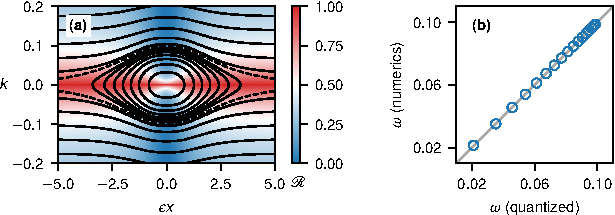
\includegraphics{localization/rod_ho.pdf}
  \end{center}
  \caption{(a) Ray trajectories for extensional waves described by the higher-order rod equations, Eq.~\eqref{eq:rod_ho}, for the sech-type curvature profile $m_{2}(x)$ [cf.~Fig.~\ref{fig:rod_bound}(b)]. (b) Bound-state frequencies obtained from numerics compared to those obtained by quantization.}
  \label{fig:rod_ho}
\end{figure}

The ray Hamiltonian for extensional and flexural waves ($\lambda_{+}$ and $\lambda_{-}$, respectively) are the two eigenvalues of $\mathsf{D}^{(0)}$, given by
%
\begin{equation}
  \lambda_{\pm}(x, k) = \frac{1}{2} \left\{\left[1 + k^2\right] \left[k^2+m^{2}(x)\right]+\sqrt{\left[k^2+1\right]^2 \left[k^2+m^{2}(x)\right]^2-4 \left[k^3-k m^{2}(x)\right]^2}\right\} - \omega^{2}.
\end{equation}
%
A simple analysis, either by plotting the rays or writing down the corresponding Hamilton's equations, reveals that even when higher-order, curvature-dependent corrections are included, flexural waves fail to form bound states, and so we focus on extensional waves instead.
Figure~\ref{fig:rod_ho}(a) shows the ray trajectories for extensional waves described by Eq.~\eqref{eq:rod_ho}.
Clearly, these rays are nearly identical to those seen previously in Fig.~\ref{fig:rod_bound}(b), showing again that the simpler rod equations are an excellent approximation to Eq.~\eqref{eq:rod_ho} in the weak curvature limit.
For the same reason, the frequencies of the extensional bound states obtained through quantization and numerics also tend to agree rather well%
\footnote{Other aspects of quantization, e.g., the lack of the extra phase $\gamma$, location of the turning points, $m^{2}(x^{\star}) = \omega^{2}$, etc., also carry over.}
with our previous results; compare, for example, Fig.~\ref{fig:rod_ho}(b) with Fig.~\ref{fig:rod_wkb}(b).

Let us conclude the discussion on rods by emphasizing that all rod models are approximate to a certain degree.
And although we have limited our analysis to just two models, we expect to see our basic result, i.e., extensional waves forming bound states around points where the absolute curvature has a minimum, in other models as well.
We next turn to wave propagation on curved shells.

\section{Waves on a curved shell}
\label{sec:shell}

One of the simplest shell theories that involve a curvature-mediated coupling between the tangential and normal components of the displacement field is the widely used Donnell--Yu shell model~\cite{donnell1933,yu1955}.
It is simple in the sense that it describes the undulations of a three-dimensional shell solely in terms of the deformation of the shell's two-dimensional midsurface, ignoring higher-order effects and retaining only the lowest-order derivatives.
For an arbitrarily parameterized midsurface, it is easiest to extract the equations of motion from the covariant form of the Donnell--Yu shell equations derived by \citet{pierce1993a}.

\subsection{Equations of motion}

We consider the middle surface of the shell to be a generalized cylinder~\cite{pressley2010} obtained by translating a plane curve $\bm{\sigma}: \mathcal{X} \to \mathbb{R}^{3}$, parameterized by $x \in \mathcal{X} \subset \mathbb{R}$, perpendicular to the plane containing it.
Thus, the shell is defined by $\bm{\Sigma}: \mathcal{X}\times\mathcal{Y} \to \mathbb{R}^{3}$, $\bm{\Sigma}(x, y) = \bm{\sigma}(x) + y{\bm{e}}_{y}$, where $\bm{e}_{y} = \partial_{y}\bm{\Sigma}$ is a constant unit vector perpendicular to the plane containing $\bm{\sigma}(x)$.
Also, $y \in \mathcal{Y}$ is the coordinate along $\bm{e}_{y}$.
For simplicity, and to make comparisons with the rod equations easier, we assume that $x$ is the arclength so that $\bm{e}_{x} = \partial_{x}\bm{\Sigma} = \bm{t}$ is the unit tangent along the curve $\bm{\sigma}$.
Furthermore, we orient $\bm{e}_{y}$ such that surface normal $\bm{e}_{x}\times\bm{e}_{y}$ coincides with the normal $\bm{n}$ to $\bm{\sigma}$.
Then, the only nonvanishing principal curvature of the shell is equal to the curve's signed curvature $m(x)$.
Propagating waves displace the shell from $\bm{\Sigma} \to \bm{\Sigma} + \delta\bm{\Sigma}$.
We write the displacement field $\delta\bm{\Sigma}$ as $\delta\bm{\Sigma} = u\bm{e}_{x} + v\bm{e}_{y} + \zeta\bm{n}$.
Assuming no external forces, the dynamic Donnell--Yu equations are
%
\begin{subequations}
  \begin{align}
    \varrho \frac{\partial^{2}\zeta}{\partial t^{2}} &= -\widetilde{B}\Delta^{2}\zeta - \widetilde{E}m^{2}(x) \zeta + \widetilde{E}m(x)\left(\frac{\partial u}{\partial x} + \eta\frac{\partial v}{\partial y}\right),\\
    \frac{\varrho}{\widetilde{E}} \frac{\partial^{2}u}{\partial t^{2}} &= -\frac{\partial\left[m(x)\zeta\right]}{\partial x} + \frac{\partial^{2}u}{\partial x^2} + \frac{(1-\eta)}{2}\frac{\partial^{2}u}{\partial y^{2}} + \frac{(1+\eta)}{2}\frac{\partial^{2}v}{\partial x \partial y},\\
    \frac{\varrho}{\widetilde{E}} \frac{\partial^{2}v}{\partial t^{2}}&= -\eta m(x)\frac{\partial \zeta}{\partial y} + \frac{(1+\eta)}{2}\frac{\partial^{2}u}{\partial x \partial y} + \frac{(1-\eta)}{2}\frac{\partial^{2}v}{\partial x^{2}} + \frac{\partial^{2}v}{\partial y^2}.
  \end{align}
\end{subequations}
%
Here $\Delta$ is the two-dimensional Laplacian, $\eta$ is the Poisson's ratio, and $\varrho$ is the density per unit area.
Also, the extensional stiffness $\widetilde{E} = Yh/(1-\eta^{2})$ and bending stiffness $\widetilde{B} = Yh^{3}/\left[12(1-\eta^{2})\right]$, with $Y$ being the Young's modulus and $h$ being the thickness of the shell.
On setting the length units to $\sqrt{\widetilde{B}/\widetilde{E}}$ and time units to $\sqrt{\smash[b]{\widetilde{B}\varrho}}/\widetilde{E}$, we arrive at the nondimensional form of these equations, which in matrix form reads
%
\begin{equation}
  \partial^{2}_{t}
  \begin{pmatrix}
    \zeta\\
    u\\
    v
  \end{pmatrix}
  +
  \widehat{\mathsf{H}}
  \begin{pmatrix}
    \zeta\\
    u\\
    v
  \end{pmatrix} = 0,\enspace
\end{equation}
%
where the operator $\widehat{\mathsf{H}}$ is defined by
%
\begin{equation}
  \widehat{\mathsf{H}} =
  \begin{pmatrix}
    \Delta^{2} + m^{2}(x) & -m(x)\partial_x & -\eta m(x) \partial_{y}\\
    m(x)\partial_{x} + m'(x) & -\partial_{x}^{2} - \frac{1}{2}(1-\eta)\partial^{2}_{y} & -\frac{1}{2}(1+\eta)\partial_{x}\partial_{y}\\
    \eta m(x)\partial_{y} & -\frac{1}{2}(1+\eta)\partial_{x}\partial_{y} & -\frac{1}{2}(1-\eta)\partial_{x}^{2} - \partial_{y}^{2}
  \end{pmatrix}.
  \label{eq:shell_wave_eq}
\end{equation}
%
A set of equations analogous to the rod equations [see Eq.~\eqref{eq:rod}] can be obtained by suppressing the $y$ derivatives in the submatrix obtained by deleting the third row and column of the operator $\widehat{\mathsf{H}}$ given above.

Translation invariance of $\widehat{\mathsf{H}}$ along $y$ lets us look for time-harmonic solutions with the common factor $e^{i(ly - \omega t)}$, where $l$ is the transverse wave number in the $y$ direction and $\omega$ is the frequency of oscillation.
This makes the wave field depend only on the coordinate $x$, and makes the transverse wave number $l$ an additional parameter of the operator $\widehat{\mathsf{H}}$.
But the operator $\widehat{\mathsf{H}}$ now has complex coefficients, and the components of its eigenmodes are complex functions.
However, while discussing the numerical results, we use a phase convention such that $\zeta, u$ are real, and $v$ is imaginary.

Similar to what we did for the rod equations, we perform a change of variables $x \to \epsilon^{-1}x$ and recast the spatial derivatives in terms of the momentum operator $\hat{k}$.
Finally, we find the dispersion matrix $\mathsf{D}^{(0)}$ as
%
\begin{equation}
\mathsf{D}^{(0)} =
\begin{pmatrix}
  (k^{2} + l^{2})^{2} + m^{2}(x) - \omega^{2} & -i k m(x) & -i\eta l m(x)\\
  ik m(x) & k^{2} + \frac{1}{2}(1-\eta)l^{2} - \omega^{2} & \frac{1}{2}(1+\eta)kl\\
  i\eta l m(x) & \frac{1}{2}(1 + \eta)kl & \frac{1}{2}(1-\eta)k^{2} + l^{2} - \omega^{2}
\end{pmatrix},\\
\end{equation}
and find its first-order correction $\mathsf{D}^{(1)}$ to be
\begin{equation}
\mathsf{D}^{(1)} =
\frac{1}{2}
\begin{pmatrix}
  0 & m'(x) & 0\\
  m'(x) & 0 & 0\\
  0 & 0 & 0
\end{pmatrix}.
\label{eq:shell_disp_matrices}
\end{equation}
%
For later analysis, it is also useful to note down the determinant%
\footnote{The expression for $\det\mathsf{D}^{(0)}$ in Eq.~\eqref{eq:shell_det} is sometimes referred to as the ``full'' dispersion relation~\cite{sondergaard2002}.  In reality, $\det\mathsf{D}^{(0)}$ is the product of three dispersion relations---a fact that we will later exploit for finding the ray trajectories.}
of $\mathsf{D}^{(0)}$, which is
%
\begin{equation}
  \begin{aligned}
    \det\mathsf{D}^{(0)} &= m^{2}(x)\left\{\left[\omega^{2} - \tfrac{1}{2}(1-\eta)l^{2}\right]\left[\omega^{2}-(1-\eta^{2})l^{2}\right] - \tfrac{1}{2}(1-\eta)k^{2}\omega^{2}\right\} \\
            &\qquad- \left[\omega^{2} - (k^{2} + l^{2})^{2}\right]
            \left[\omega^{2} - \tfrac{1}{2}(1-\eta)(k^{2} + l^{2})\right]
            \left[\omega^{2} - (k^{2} + l^{2})\right].
  \end{aligned}
  \label{eq:shell_det}
\end{equation}
%
Before we continue, it is insightful to examine the dispersion relations for plain waves propagating on singly-curved shells of constant curvature.

\subsection{Shells of constant curvature}

First we analyze the zero curvature limit, i.e., when the shell becomes a flat plate.
In this limit, the wave equation, Eq.~\eqref{eq:shell_wave_eq}, decouples into two equations, the first of which involves only the normal component $\zeta$, and represents flexural waves.
The second equation, representing extensional and shear waves, only involves the tangential components $u$ and $v$.
Shear waves propagate transversely to the in-plane wave vector $k\bm{e}_{x} + l\bm{e}_{y}$, whereas extensional waves are longitudinal to it.
Setting $m = 0$ in Eq.~\eqref{eq:shell_det}, we find the following flat-plate dispersion relations
%
\begin{equation}
  \omega_{0}^{2} = \left(k^{2} + l^{2}\right)^{2},\quad
  \omega_{0}^{2} = \frac{1}{2}\left(1-\eta\right)\left(k^{2} + l^{2}\right),
  \quad\text{and}\quad
  \omega_{0}^{2} = \left(k^{2} + l^{2}\right),
  \label{eq:shell_disp_zero}
\end{equation}
%
which we recognize as the dispersion relations of flexural, shear, and extensional waves, respectively~\cite{fung1965}.
The above dispersion relations for a fixed transverse wave number $l$ are indicated by the dashed black curves in Fig.~\ref{fig:shell_disp}.
Because $l$ is nonzero, there is now a gap in the dispersion curves and a corresponding nonzero cut-on frequency for each of these waves.
%
\begin{figure}
  \begin{center}
    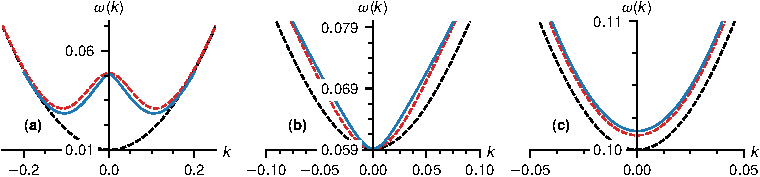
\includegraphics{localization/shell_disp.pdf}
  \end{center}
  \caption{%
    Dispersion curves for plain waves propagating on a cylinder of constant curvature $m = 0.05$ for (a) flexural, (b) shear, and (c) extensional waves.
    In each plot, the solid blue curves represent the actual dispersion curves obtained by finding $\omega$ using Eq.~\eqref{eq:shell_cubic_sol}.
    The dashed red curves represent the approximate dispersion relation in Eq.~\eqref{eq:shell_disp_approx}.
    Also, the dashed black curves indicate the dispersion curves for an uncurved flat plate, i.e., when $m = 0$ [Eq.~\eqref{eq:shell_disp_zero}].
    The transverse wave number $l = 0.1$ and Poisson's ratio $\eta = 0.3$ for all curves.
  }
  \label{fig:shell_disp}
\end{figure}

\subsubsection*{Exact dispersion relations}

For nonzero but constant curvature, plain waves continue to propagate on the shell, which now becomes part of a thin cylinder.
For simplicity, we shall continue to call these waves as being flexural, extensional, or shear in nature.
However, as with the curved rod, we expect some amount of mixing of the tangential and normal displacements due to nonzero curvature.
Also, to find the dispersion relations from Eq.~\eqref{eq:shell_det} we now need to use the general cubic formula~\cite{olver2010}, which results in unwieldy analytical expressions.
More specifically, these relations can be obtained by solving the following cubic in $\omega^{2}$:
%
\begin{equation}
  \omega^{6} - a\omega^{4} - b\omega^{2} - c = 0
\end{equation}
%
where the coefficients
%
\begin{equation}
  \begin{aligned}
    a &= \frac{1}{2}q^{2}\left[(3 - \eta) + 2q^{2}\right],\\
    b &= -\frac{1}{2}q^{4}\left[(3 - \eta)q^{2} + (1 - \eta)\right] - \frac{1}{2}m^{2}(1 - \eta)\left[q^{2} + 2(1 + \eta)l^{2}\right],\\
    c &= \frac{1}{2}(1-\eta)\left[q^{8} + m^{2}l^{4}\left(1 - \eta^{2}\right)\right],
  \end{aligned}
\end{equation}
%
and $q^{2} = k^{2} + l^{2}$ is the magnitude of the wave vector.
The above cubic has the solution
%
\begin{equation}
  \omega^{2} =
  \begin{dcases}
    \frac{1}{3}a + \frac{2^{1/3}\left(a^{2} + 3b\right)}{3d} + \frac{d}{3\times2^{1/3}} & \text{(extensional)},\\
    \frac{1}{3}a - \frac{\left(1 - i\sqrt{3}\right)\left(a^{2} + 3b\right)}{3\times2^{2/3}d} - \frac{\left(1 + i\sqrt{3}\right)d}{6\times2^{1/3}} & \text{(shear)},\\
    \frac{1}{3}a - \frac{\left(1 + i\sqrt{3}\right)\left(a^{2} + 3b\right)}{3\times2^{2/3}d} - \frac{\left(1 - i\sqrt{3}\right)d}{6\times2^{1/3}} & \text{(flexural)}.\\
  \end{dcases}
  \label{eq:shell_cubic_sol}
\end{equation}
%
where
%
\begin{equation}
  d = \left(2 a^3+9 a b+27 c+3 \sqrt{3}\sqrt{4 a^3 c-a^2 b^2+18 a b c-4 b^3+27 c^2}\right)^{1/3}.
\end{equation}
%
It is not directly obvious how the roots in Eq.~\eqref{eq:shell_cubic_sol} can be associated with a specific wave polarization.
To do so, we have to take the limit $m \to 0$ numerically and find which of the roots reduce to the flat-plate results in Eq.~\eqref{eq:shell_disp_zero}.

As an example, using Eq.~\eqref{eq:shell_cubic_sol}, we find the dispersion curves at a curvature value of $m = 0.05$, which are indicated by the solid lines in Fig.~\ref{fig:shell_disp}.
We make two observations on comparing these curves with the dispersion curves for a flat plate:
(i) the gap in the dispersion curves for flexural and extensional waves [Figs.~\ref{fig:shell_disp}(a) and~\ref{fig:shell_disp}(c)] have increased, and the flexural dispersion curve now has a double-well appearance;
(ii) although the dispersion curve for shear waves has changed in appearance [Fig.~\ref{fig:shell_disp}(b)], the gap remains the same and the cut-on frequency remains unchanged.
The cut-on frequencies at nonzero $m$ can be computed from Eq.~\eqref{eq:shell_det} after setting $k = 0$, and we find three roots
%
\begin{equation}
  \omega^{2}_{\text{cut-on}} =
    \frac{1}{2}\left(l^{2} + l^{4} + m^{2} \pm \sqrt{\left(l^{2} - l^{4} - m^{2}\right)^{2} + 4\eta^{2}l^{2}m^{2}}\right)
    \quad\text{and}\quad
    \frac{1}{2}(1-\eta)l^{2}.
    \label{eq:shell_cuton}
\end{equation}
%
Our intuition and a series expansion in $m$ suggests that the lowest of the first two roots must be associated with flexural waves and the highest root must be associated with extensional waves.
The third root, which is independent of the curvature $m$, must then correspond to the cut-on frequency for shear waves.
As we shall see, this association is only correct at very low curvatures.

\subsubsection*{Approximate dispersion relations}

Although the exact dispersion relations for nonzero curvature are unwieldy, we can find an approximate expression for the dispersion relations in the very weak curvature limit.
To this end, we write the roots $\omega^{2}$ as a regular perturbation series~\cite{bender1978} in even powers of $m$, i.e.,
%
\begin{equation}
  \omega^{2}(k, l) = \omega^{2}_{0}(k, l) + \sum_{n = 1}^{\infty} m^{2n}Q_{n}(k, l),
  \label{eq:shell_perturb}
\end{equation}
%
where $\omega_{0}$ is one of the three roots in Eq.~\eqref{eq:shell_disp_zero} and $Q_{n}(k, l)$ are coefficients to the correction terms that we have to determine.%
\footnote{Note that it is a futile task to expand the roots in Eq.~\eqref{eq:shell_cubic_sol} in powers of $m$ to find the approximate dispersion relationships.}
Since the curvature is assumed to be very weak, the dispersion relations obtained this way can be associated with a wave type based on the choice we make for $\omega_{0}$.
Putting Eq.~\eqref{eq:shell_perturb} in Eq.~\eqref{eq:shell_det}, and dropping powers of $k$ and $l$ in comparison to unity, we find
%
\begin{equation}
  \omega^{2} =
  \begin{dcases}
    \left(k^{2} + l^{2}\right)^{2} + \left(1 - \eta^{2}\right)m^{2}\frac{l^{4}}{\left(k^{2} + l^{2}\right)^{2}} + \mathcal{O}(m^{4}) & \text{(flexural)}, \\
    \frac{1}{2}\left(1-\eta\right)\left(k^{2} + l^{2}\right) + 2\left(1 - \eta\right)m^{2}\frac{k^{2}l^{2}}{\left(k^{2} + l^{2}\right)^{2}} + \mathcal{O}(m^{4}) & \text{(shear)},\\
    (k^{2} + l^{2}) + m^{2}\frac{\left(k^{2} + \eta l^{2}\right)^{2}}{\left(k^{2} + l^{2}\right)^{2}} + \mathcal{O}(m^{4}) & \text{(extensional)}.
  \end{dcases}
  \label{eq:shell_disp_approx}
\end{equation}
%
The above approximate dispersion relations are identical to those found in the literature and derived using alternative approaches~\cite{germogenova1973,pierce1993,norris1994,rebinsky1996}.
Also, in their analytical characterization of bound waves in a musical saw, \citet{shankar2022} works exclusively with the above approximate dispersion relation for flexural waves, which has also been observed experimentally~\cite{williams1990}.
In Fig.~\ref{fig:shell_disp}, the approximate dispersion relations for $m = 0.05$ are indicated by the red dashed curves, from which we can see that Eq.~\eqref{eq:shell_disp_approx} captures the true dispersion relations to a reasonably good accuracy.

Equation~\eqref{eq:shell_disp_approx} must break down beyond a certain value of the curvature.
Indeed, we only expect it to capture the true dispersion when the $\mathcal{O}(m^{2})$ correction term in Eq.~\eqref{eq:shell_perturb} is smaller than $\omega_{0}^{2}$, and more conservatively, only when $m \ll k^{2} + l^{2}$.
We would expect the dispersion relation to deviate significantly from Eq.~\eqref{eq:shell_disp_approx} as $m$ increases.
In fact, for small $k$ and $l$, Eq.~\eqref{eq:shell_disp_approx} completely breaks down at a curvature at which the cut-on frequency for flexural and extensional waves become equal.
For nonzero $l$, from Eq.~\eqref{eq:shell_cuton}, we see that this happens at a curvature value
%
\begin{equation}
  m_{\ddag}^{2} = \frac{(1 + \eta)l^{2}\left[\frac{1}{2}(1 - \eta) - l^{2}\right]}{\left(1 + 2\eta\right)\left(1 - \eta\right)}
  = \frac{1}{2}\left(\frac{1+\eta}{1 + 2\eta}\right)l^{2} + \mathcal{O}(l^{4}).
  \label{eq:shell_mdag}
\end{equation}
%
We graphically demonstrate this in Fig.~\ref{fig:shell_gap}, from which we can see that the expressions for the cut-on frequencies for shear and flexural waves get interchanged at large $m$.
Hence, for $m > m_{\ddag}$, the lowest of the first two cut-on frequencies in Eq.~\eqref{eq:shell_cuton}, should be associated with shear waves, whose dispersion curves would now have a curvature-dependent gap.
The cut-on frequency for flexural waves, however, would now be equal to $\frac{1}{2}(1-\eta)l^{2}$.
We remark that this switching of the cut-on frequencies does not happen if $l^{2} > \frac{1}{2}(1-\eta)$ as Eq.~\eqref{eq:shell_mdag} fails to have a real root.
Also, as the cut-on frequencies of flexural and shear waves are equal for $m = m_{\ddag}$, in principle, mode conversion can occur close to the entire $k$ axis on the phase plane.
Despite such a possibility, we did not observe any discernible effects of mode conversion in our numerical experiments, and we shall it ignore in our analysis.
%
\begin{figure}
  \begin{center}
    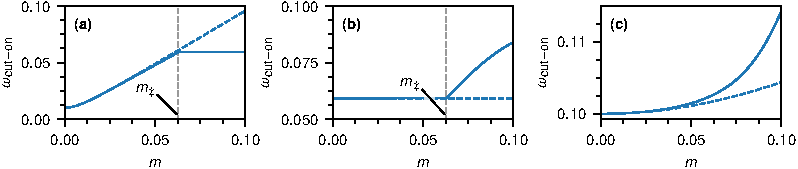
\includegraphics{localization/shell_gap.pdf}
  \end{center}
  \caption{%
    Cut-on frequencies for a singly-curved shell as a function of the curvature $m$ for (a) flexural, (b) shear, and (c) extensional waves.
    The blue dashed curves represent the cut-on frequency predicted by Eq.~\eqref{eq:shell_disp_approx}, which holds only when $m$ is small.
    The solid curves represent the actual cut-on frequency obtained by finding $\omega$ from Eq.~\eqref{eq:shell_det} using the general cubic formula, and taking the limit $k \to 0$ numerically.
    The transverse wave number $l = 0.1$ and Poisson's ratio $\eta = 0.3$ in all plots.
  }
  \label{fig:shell_gap}
\end{figure}

\subsection{Shells with varying curvature}

We shall now consider singly-curved shells with varying curvature profiles.
Given the complexity of the general dispersion relations and the myriad of subtleties, we shall, however, perform a less exhaustive analysis compared to what we did for the rod.
We shall only look at a limited number of examples, and to simplify matters, we set the transverse wave number $l = 0.1$ and Poisson's ratio $\eta = 0.3$ (corresponding to that of steel) throughout.
As for the rod, we will consider both tanh-type and sech-type curvature profiles, but we assume that the largest absolute curvature $b > m_{\ddag}$.
This would let us examine the problem beyond the range of validity of the approximate dispersion relation in Eq.~\eqref{eq:shell_disp_approx}.
For the sech-type curvature profile, we additionally assume that the smallest curvature $a < m_{\ddag}$.
With $l = 0.1$ and $\eta = 0.3$, we have $m_{\ddag} \approx 0.06$, and these assumptions are satisfied by the choices $a = 0.01$ and $b = 0.1$ that we made for the rod, and we use them for the shell as well.

From our earlier analysis, we saw that the spectral gap in the dispersion relation for all three wave polarizations grows with increasing curvature.
Now, consider a wave traveling from a region of low curvature to one of high curvature.
As the wave moves, at some point, the frequency of the wave would fall below the local cut-on frequency of waves, where it gets reflected back.
Intuitively, we therefore expect bound states to occur for all three wave polarizations.
%
\begin{figure}
  \begin{center}
    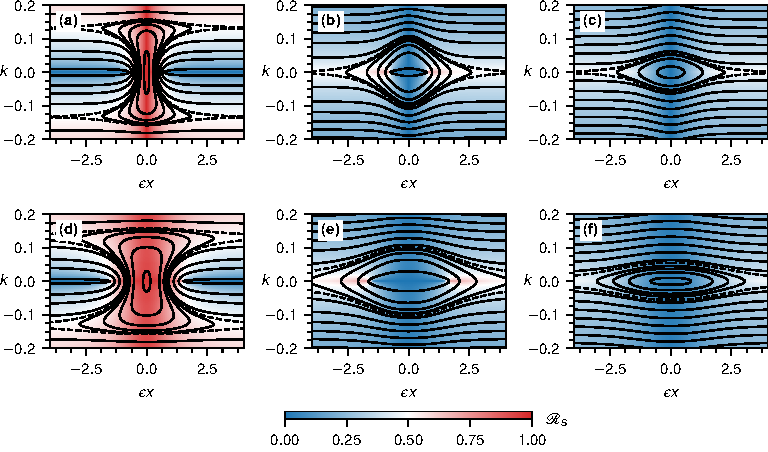
\includegraphics{localization/shell_rays.pdf}
  \end{center}
  \caption{%
    Rays trajectories for a curved shell with a tanh-type curvature profile (top panels) and a sech-type curvature profile (bottom panels) showcasing (a), (d) flexural waves, (b), (e) shear waves, and (c), (f) extensional waves.
    In all figures the closed curves represent rays associated with quantized bound states and the dashed black curves represent the highest frequency for which there is a bound state.
    The phase portraits have also been color coded with the ratio $\mathscr{R}_{s}$ defined in Eq.~\eqref{eq:shell_ratio}.
  }
  \label{fig:shell_rays}
\end{figure}

For ray analysis, we usually directly work with the eigenvalues of the dispersion matrix $\mathsf{D}^{(0)}$.
This proves to be difficult for the shell as the expressions for the eigenvalues are unwieldy.
In the absence of mode conversion, however, only one eigenvalue, say $\lambda$, will vanish at a given phase-space point $(x, k)$, causing the determinant $\det\mathsf{D}^{(0)}$ to vanish as well.
Hence, the rays determined by $\lambda(x, k; \omega) = 0$ and $\det\mathsf{D}^{(0)} = 0$ are identical, allowing us to use $\det\mathsf{D}^{(0)}$ as the ray Hamiltonian.%
\footnote{Let us remark that the ray trajectories can also be obtained by treating $\omega^{2}$ in Eq.~\eqref{eq:shell_cubic_sol} as the ray Hamiltonian.  However, given the general awkwardness of the expressions, it is better to work with $\det\mathsf{D}^{(0)}$ instead.}
Using $\det\mathsf{D}^{(0)}$ instead of $\lambda$ would amount to a trivial reparameterization of Hamilton's equations~\cite{tracy2014}.
Judicious choices of the initial conditions, i.e., the coordinates $(x, k)$ and frequency $\omega$, obtained from the local dispersion curves at a given $(x, k)$, would determine the type of wave the ray represents.
When analyzing a given wave type, it is also useful to compute an amplitude ratio, analogous to the one we used for the curved rod, and defined by
%
\begin{equation}
  \mathscr{R}_{s} = \frac{\abs{\zeta}}{\abs{\zeta} + \abs{u} + \abs{v}} \sim \frac{\abs{\tau_{1}}}{\abs{\tau_{1}} + \abs{\tau_{2}} + \abs{\tau_{3}}}.
  \label{eq:shell_ratio}
\end{equation}
%
Above, we have also made use of the fact that the wave field is asymptotic to the polarization vector $\tau$ to write $\mathscr{R}_{s}$ in terms of the components of $\tau$.
With the above definition, flexural waves in a flat plate have $\mathscr{R}_{s} = 1$, whereas both shear and extensional waves have $\mathscr{R}_{s} = 0$.
In a curved shell, because we expect both the normal and tangential components of the wave field to be significant, $\mathscr{R}_{s}$ for the three wave polarizations would deviate from their flat-plate counterparts.
For all three wave types, a significant amount of normal and tangential contribution to the displacement field is indicated by values of $\mathscr{R}_{s}$ in the range $1/3 < \mathscr{R}_{s} < 1/2$.
We discuss flexural waves first.

\subsubsection*{Flexural waves}
\label{sec:shell_flexural}

Our intuitive expectation of flexural bound states is confirmed by the actual ray trajectories for flexural waves showcased in Figs.~\ref{fig:shell_rays}(a) and~\ref{fig:shell_rays}(d).
For frequencies slightly above the cut-on frequency at $x = 0$, the rays appear in the form of closed, vertically-elongated orbits that remain confined to a region where the curvature is very small.
At larger frequencies, the rays begin to enter regions of higher curvature, and orbits change from being elliptical to highly eccentric, ``peanut''-shaped curves.
For these orbits, we have a total of six caustics where $\dot{x} = 0$.
[Compare Figs.~\ref{fig:shell_rays}(a) and~\ref{fig:shell_rays}(d) with Fig.~\ref{fig:caustic}(b).]
Two of these caustics, which are on the $x$ axis, are the usual classical turning points where $k = 0$.
At the other four caustics $k \neq 0$, and they arise due to the two double-well minima in the (local) dispersion curves where $\dd{\omega}/\dd{k} = 0$.

For the peanut-shaped orbits, bound states do not occur beyond a frequency where the four caustics with $k \neq 0$ get pushed to $x = \pm \infty$.
Since the absolute curvature $\abs{m(\pm \infty)} = b$ for both curvature profiles, the largest frequency for which we see a bound state---represented by the dashed rays in Figs.~\ref{fig:shell_rays}(a) and~\ref{fig:shell_rays}(d)---must be the frequency of the double-well minimum in the dispersion curves for $m = b$.
For small enough $b$, using Eq.~\eqref{eq:shell_disp_approx}, we find this minimum to be $\omega^{2} \approx 2\sqrt{l^{4}b^{2}(1-\eta^{2})}$.
This expression, however, turns out to overestimate the actual minimum for larger $b$, and we must find it numerically.
Also, this minimum exists only when $b \gtrsim l^{2}/\sqrt{1-\eta^{2}}$.
For smaller $b$, rays of the bound states remain elliptical in nature, with the classical turning points being the only caustics.

An example profile of a low-frequency flexural bound state is shown in Fig.~\ref{fig:shell_modes_tanh}(a).
This state has negligible tangential components $u$ and $v$, and remains confined to a region of similar extent as the classical turning points.
At higher frequencies, flexural bound states grow beyond the classical turning points and enter regions of higher curvature.
Here curvature effects become more prominent, and the states tend to have both tangential and normal components as seen from Fig.~\ref{fig:shell_modes_tanh}(b), and the color coding of the phase portraits.
They, however, remain confined to a region of similar extent as the four caustics with $\dot{x} = 0$.
%
\begin{figure}
  \begin{center}
    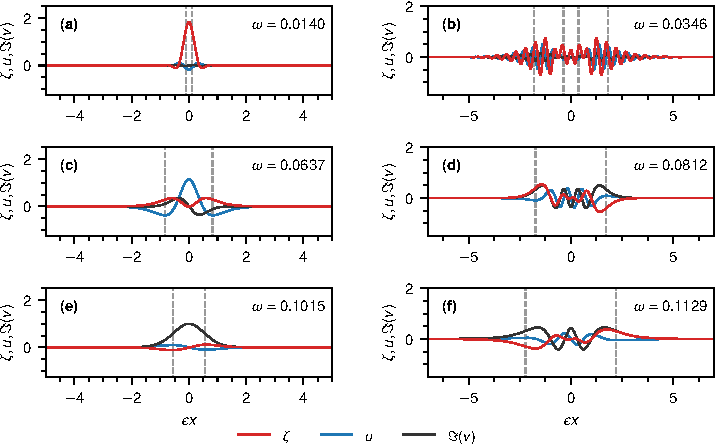
\includegraphics{localization/shell_modes_tanh.pdf}
  \end{center}
  \caption{
  Numerical eigenmodes of a curved shell with a tanh-type curvature profile showing (a),(b) flexural, (c),(d) shear, and (e),(f) extensional bound states.
  In our phase convention, $\zeta$ and $u$ are always real, whereas $v$ is always complex, which is why we only show its imaginary component $\Im(v)$.
  Left panels depict low-frequency bound states, whereas the ones on the right panels have a higher frequency.
  The dashed vertical lines indicate the locations of the caustics.
}
  \label{fig:shell_modes_tanh}
\end{figure}

\subsubsection*{Shear waves}

From the phase portraits in Fig.~\ref{fig:shell_rays}(b) and~\ref{fig:shell_rays}(e), we see that shear waves also form bound rays confined between two classical turning points.
As the frequency of the orbits increase, the turning points move to $x = \pm \infty$, where the absolute curvature for both curvature types is $b$.
Thus, the largest frequency for which we observe shear bound states is the shear-wave cut-on frequency for a cylindrical shell of curvature equal to $b$, obtained by setting $m = b$ in the second root of Eq.~\eqref{eq:shell_cuton}.
Beyond this frequency, shear waves form unbound states.
The rays of shear bound states are elongated along the $x$ direction as the spectral gap in the local dispersion curve does not begin increasing until $m(x) > m_{\ddag}$.
For the same reason, shear waves do not get localized if $b < m_{\ddag}$.
It is then natural to wonder if the localization of shear waves seen in the phase portraits is an artifact of having chosen a relatively large value of $b = 0.1$.
But from Eq.~\eqref{eq:shell_mdag} we see that $m_{\ddag}$ can be made arbitrarily small by adjusting the value of transverse wave number $l$, so that even for small $b$ we would expect shear bound states.

Example profiles of two shear bound states are shown in Figs.~\ref{fig:shell_modes_tanh}(c) and~\ref{fig:shell_modes_tanh}(d).
The first one has a frequency that is only slightly above the shear-wave cut-on frequency and hence its local wave number $k$ is small.
Therefore, its (local) wave vector is predominantly in the $y$ direction [see Fig.~\ref{fig:waves}(b)].
Furthermore, as expected from the transverse nature of shear waves, the dominant tangential component is $u$, which is the displacement along $x$.
The second shear bound state shown in Fig.~\ref{fig:shell_modes_tanh}(f) has a higher frequency, causing it to spread to regions of higher curvature, where curvature effects become more prominent.
This can also be inferred from the color coding of Figs.~\ref{fig:shell_rays}(b) and~\ref{fig:shell_rays}(e), which shows that shear bound states develop a significant normal component at higher frequencies.

\subsubsection*{Extensional waves}

Color-coded phase portraits of extensional waves indicating bound states are shown in Figs.~\ref{fig:shell_rays}(c) and~\ref{fig:shell_rays}(f).
The caustics for these bound states are the usual classical turning points with $k=0$.
For higher-frequency bound states, these points move to $\pm \infty$, where the absolute curvature is $b$.
Hence, the largest frequency for which we observe extensional bound states must be the cut-on frequency for extensional waves in a shell having a curvature equal to $b$, obtained by putting $m = b$ in the first root in Eq.~\eqref{eq:shell_cuton}.

Example profiles of two extensional bound states are shown in Figs.~\ref{fig:shell_modes_tanh}(e) and~\ref{fig:shell_modes_tanh}(f).
Low-frequency extensional bound states, such as the one in Fig.~\ref{fig:shell_modes_tanh}(e), are expected to displace the shell predominantly in the $y$ direction as seen from the comparatively large values of the tangential component $v$.
The bound state in Fig.~\ref{fig:shell_modes_tanh}(f) has a slightly higher frequency, causing it to spread to regions of higher curvature, where it develops a significant normal component, which we also infer from the color coding of Figs.~\ref{fig:shell_rays}(c) and~\ref{fig:shell_rays}(f).

\subsubsection*{Bound states and quantization}

To find the bound-state frequencies, we first set $k=0$ in Eq.~\eqref{eq:shell_det} and rearrange terms to find that that classical turning points $x^{\star}$ are given by the solutions to the implicit equation
%
\begin{equation}
  m^{2}(x^{\star}) = \left[\frac{\omega^{2} - l^{2}}{\omega^{2} - \left(1-\eta^{2}\right)l^{2}}\right]\left(\omega^{2}-l^{4}\right).
  \label{eq:shell_caustic}
\end{equation}
%
Depending on the value of $\omega$, the turning points found using the above equation could correspond to turning points on the bound rays of all three waves.
We use the same quantization procedure as for the rod to determine the bound-state frequencies (Appendix~\ref{app:numerical}).
Furthermore, the extra phases $\gamma_{\text{G}}$ and $\gamma_{\text{NG}}$ in the quantization condition in Eq.~\eqref{eq:quantization} vanish for the shell equations as well (Appendix~\ref{app:additional_phase}).
The Keller--Maslov index continues to be $\alpha = 2$ for all orbits---including the peanut-shaped orbits with six caustics---as they can be smoothly deformed into a circle centered around the origin~\cite{percival1977}.
From Fig.~\ref{fig:shell_wkb}, we see that the bound-state frequencies obtained through quantization agree rather well with the numerical values for both curvature profiles.
% Also, from Fig.~\ref{fig:shell_rays} we see that the sech-type orbits generally enclose a larger area compared to the tanh-type orbits.
% Hence, it is not surprising that a sech-type shell possesses more bound states for all three wave polarizations.
%
\begin{figure}
  \begin{center}
    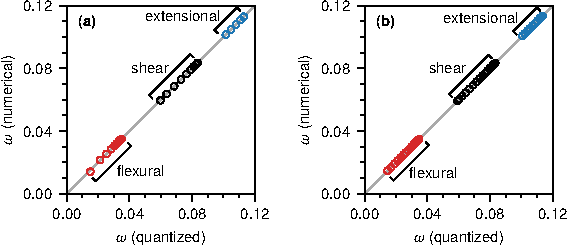
\includegraphics{localization/shell_wkb.pdf}
  \end{center}
  \caption{
    Bound-state frequencies of a curved shell obtained from numerics compared to that obtained through quantization for (a)
    tanh-type curvature profile $m_{1}(x)$ and (b) sech-type curvature profile $m_{2}(x)$.
    For both plots, the gray guide line in the background represents $\omega$ (quantized) = $\omega$ (numerical).
  }
  \label{fig:shell_wkb}
\end{figure}

Although waves of all three types form bound states, from our preceding analyses and Fig.~\ref{fig:shell_wkb}, we see that flexural bound states appear first, followed by shear and extensional bound states.
Thus, in very long shells, shear waves form bound states that lie in a quasi-continuum of flexural waves spread across the shell.
Likewise, extensional bound states would lie in a quasi-continuum of unbound flexural and shear waves.
Similar to the curved rod, the bound states of the curved shell are also of definite parity when the curvature profile $m(x)$ is odd or even.
More specifically, when $m(x)$ is even, the components $\zeta(x)$ and $v(x)$ have the same parity, with $u(x)$ having the opposite parity.
For odd $m(x)$, however, $\zeta(x)$ and $u(x)$ have the same parity, with $v(x)$ having the opposite parity, as can be seen from the example bound states in Fig.~\ref{fig:shell_modes_tanh}.

% Parity analysis
% ---------------
%
% Let also remark that the bound states of all three wave polarizations are also of definite parity when the curvature $m(x)$ is odd or even.
% From Eq.~\eqref{eq:shell_wave_eq}, we can verify that for an odd $m(x)$, if $\psi(x) = \left[\zeta(x), u(x), v(x)\right]$ is an eigenmode, then $\psi(x) = \left[\zeta(-x), u(-x), -v(-x)\right]$ is an eigenmode as well.
% Assuming nondegeneracy, this implies that the real and complex components of $\zeta(x)$ and $u(x)$ have the same parity, i.e., they are both odd or both even.
% The components of $v(x)$, however, would have the opposite parity.
% For the odd tanh-type curvature profile, we see this in Figs.~\ref{fig:shell_modes_tanh}(a)--(c), where $\zeta(x)$ and $u(x)$ are even, and $\Im\left[v(x)\right]$ is odd.
% Similarly, in Figs.~\ref{fig:shell_modes_tanh}(d)--(f), we observe that $v(x)$ is even, and $\zeta(x)$ and $u(x)$ are odd.
% A similar analysis reveals that for an even $m(x)$, the components of $\zeta(x)$ and $v(x)$ have the same parity, with the components of $u(x)$ having the opposite parity.

\section{Shells with sharp bends}

Flexural bound states have also been predicted to exist in curved shells around points of maximal curvature~\cite{mohammed2021}.
To illustrate this, we consider the curvature profile%
\footnote{The authors of Refs.~\cite{sondergaard2002,mohammed2021} use a much more complicated curvature profile in their analysis.  However, for our purposes, $m_{3}(x)$ has the basic features of the profiles that these authors consider.}
$m_{3}(x) = b\sech(\epsilon x)$.
For the parameter values $b = 0.1$ and $\epsilon = 0.01$, Fig.~\ref{fig:shell_m3_profile} shows the function $m_{3}(x)$ and the shape of a curve with this curvature profile.
Clearly, the curve intersects itself at multiple points, and hence $m_{3}(x)$ can only be the curvature profile of a physically unrealizable ``phantom'' shell that allows self intersections.
Although self intersections can be avoided by choosing a smaller value for $b$ (or a larger value for $\epsilon$), doing so would lead to the formation of very few or barely discernible bound states.
For this reason, we will continue to work with the choice $b=0.1$ so that the bound states appear more conspicuous, enabling us to better test our conclusions from a semiclassical analysis.
%
\begin{figure}
  \begin{center}
    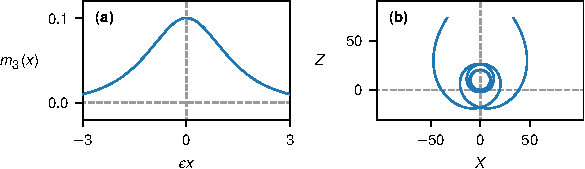
\includegraphics{localization/m3_sech_profile.pdf}
  \end{center}
  \caption{%
    (a) Curvature profile $m_{3}(x) = b\sech{\epsilon x}$ and (b) a curve with this curvature profile in Cartesian space with coordinates $X$ and $Z$.
    As the curve has multiple self intersections, only a physically unrealistic ``phantom'' shell can have this curvature profile.
    The parameters $b = 0.1$ and $\epsilon = 0.01$.
  }
  \label{fig:shell_m3_profile}
\end{figure}

Ray trajectories of all three wave types for the curvature profile $m_{3}(x)$ are shown in Fig.~\ref{fig:shell_m3_rays}.
As we see from this figure, only flexural waves form bound states.
For this reason, we forgo a more detailed analysis of shear and extensional waves, and concentrate on flexural waves alone.
In the phase portrait of Fig.~\ref{fig:shell_m3_rays}(a), we see that in addition to the nonlinear center at the origin, there are two saddle points on the $k$ axis.
The saddle points arise because of the double-well minimum in the flexural dispersion curves where $\dd{\omega}/\dd{k} = 0$.
A more detailed analysis of the phase portraits and bound states of flexural waves reveals the following:
%
\begin{enumerate}
  \item
    The existence of bound states around regions of high curvature cannot simply be explained by considering the gap and/or cut-on frequency in the dispersion curves---after all, as we move away from regions of high curvature to regions of low curvature, this gap decreases.
    In reality, these bound states arise due to the double-well nature of the flexural dispersion curves at nonzero curvature.
    Indeed, if $l = 0$ or $b \lesssim l^{2}/\sqrt{\smash[b]{1-\eta^{2}}}$, the dispersion curves fails to have a double-well nature and bound states do not exist.%
    \footnote{This should be contrasted with flexural bound states around points of minimal curvature, which continue to exist even for $b \lesssim l^{2}/\sqrt{\smash[b]{1-\eta^{2}}}$; see the discussion on p.~\pageref{sec:shell_flexural}.}
  \item Smaller orbits in the phase portraits represent bound states of \emph{higher} frequency.
    Hence, higher-frequency bound states are represented by a smaller quantum number $n$.
    The smallest bound orbit has a frequency slightly above the cut-on frequency of flexural waves at curvature $m = b$.
    For $b > m_{\ddag}$, as the frequency of the orbit approaches the cut-on frequency, the whole orbit flattens to a small line segment on the $x$ axis; for $b < m_{\ddag}$, the orbit shrinks to the origin. [See Eq.~\eqref{eq:shell_mdag} for the definition of $m_{\ddag}$.]
  \item As the frequency of the bound orbits gets smaller, they increase in size, but remain confined between the two heteroclinic orbits [shown as dashed curves in Fig.~\ref{fig:shell_m3_rays}(a)] connecting the saddle points on the $k$ axis.
    The heteroclinic orbits have a frequency equal to the double-well minimum in the dispersion curves, which puts a limit on the \emph{lowest} frequency for which we expect a bound mode.
  \item Incoming and outgoing rays close to the saddle point are nearly tangent to each other, leading to the formation of a tunneling region around the saddle point.%
    \footnote{\citet{mohammed2021} presents a detailed analysis of this tunneling phenomenon.}
    In this region, waves represented by one ray can transfer their energy to waves represented by the other ray~\cite{tracy2014}, which causes the lower-frequency bound states to ``leak out'' as shown in Fig.~\ref{fig:shell_m3_results}(a).
    This, however, does not seem to have a considerable effect on the quantization results, and we recover the frequencies of the observed bound modes accurately [see Fig.~\ref{fig:shell_m3_results}(c)].
  \item Finally, bound states at higher frequencies, such as the one in Fig.~\ref{fig:shell_m3_results}(b), tend to have fewer nodes and appear to be more spatially confined.%
    \footnote{This is in contrast to all the bound states, including those on the curved rod, that we have described so far.}
    They also have more significant tangential contribution as evident from the color coding of Fig.~\ref{fig:shell_m3_rays}(a).
\end{enumerate}
%
\begin{figure}
  \begin{center}
    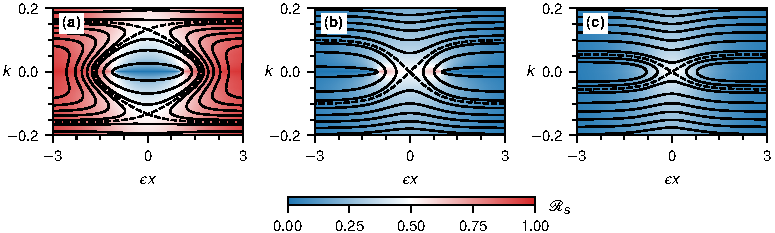
\includegraphics{localization/shell_rays_altsech.pdf}
  \end{center}
  \caption{%
    Rays trajectories for a curved shell with the curvature profile $m_{3}(x)$ showing (a) flexural waves, (b) shear waves, and (c) extensional waves.
    Only flexural waves form bound states.
    The phase portraits are color coded with the ratio $\mathscr{R}_{s}$ defined in Eq.~\eqref{eq:shell_ratio}.
  }
  \label{fig:shell_m3_rays}
\end{figure}

In summary, flexural bound states in a shell can also develop around points of maximal curvature.
Let us again remark, however, that for the parameter choices $b = 0.1$ and $\epsilon = 0.01$, the curvature profile $m_{3}(x)$ is a physical unrealizable one.
On the other hand, numerical experiments with more realistic shells (with small $b$ and/or large $\epsilon$) revealed very few or practically nonexistent bound states---something that we expect to happen in real experiments as well.

\begin{figure}
  \begin{center}
    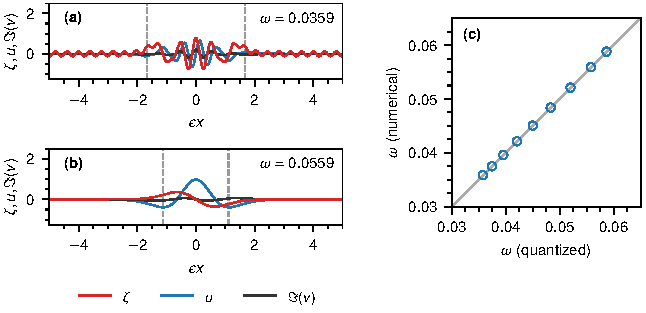
\includegraphics{localization/shell_altsech_results.pdf}
  \end{center}
  \caption{%
    (a), (b) Example flexural bound states for a shell with curvature profile $m_{3}(x)$; the grey vertical lines indicate the locations of the classical turning points.
    Tunneling effects around the saddle points cause the lower-frequency modes, such as the one in~(a), to leak out.
    (c) Comparison between the quantization results and numerics; the grey guideline in the background represents $\omega~\text{(quantized)} = \omega~\text{(numerical)}$.
  }
  \label{fig:shell_m3_results}
\end{figure}

\section{Concluding remarks}
\label{sec:conclusion}

In this chapter we have considered the localization of waves in thin elastic structures induced by variations in the structure's curvature profile.
For both the example structures we considered, bound states develop around points where the structure's absolute curvature has a minimum.
In case of the shell, flexural, shear, and extensional waves form bound states.
Additionally, flexural bound states can also develop around points of a shell where the absolute curvature has a maximum.
In contrast to shells, bound states in a curved rod (which are always extensional in nature) only exist around points where the absolute curvature has a minimum.
These findings set the stage for the design of simple devices capable of inducing wave localization without relying on metamaterials with nontrivial microstructure.

Semiclassical approximation presents challenges of its own when used to study multicomponent waves, particularly due to the presence of nontrivial phases in the quantization rule.
The rod and shell equations we use in this paper, however, have properties that cause these phases to vanish.
Nevertheless, topologically protected waves in continuous media can arise when this phase is nonzero, especially when time-reversal symmetry is broken~\cite{venaille2023}.
For this reason, it is worthwhile to explore the use of semiclassical methods in problems with broken time-reversal symmetry such as those in rotating elastic media~\cite{marijanovic2022}, fluids with odd viscosity~\cite{souslov2019}, and magnetoelastic waves~\cite{banos1956}, where one would generically expect this phase to be nonzero.

\begin{subappendices}

\section{Additional phases}
\label{app:additional_phase}

In this appendix we will look at situations where the extra phase $\gamma$ that appears in the quantization condition in Eq.~\eqref{eq:quantization} vanishes.
As we described in the main text, $\gamma = \gamma_{\text{G}} + \gamma_{\text{NG}}$, where $\gamma_{\text{G}}$ is the term that gives rise to a nonzero geometric phase and $\gamma_{\text{NG}}$ is the other (non-geometric) term.
First, we shall analyze general $N$-component wave equations with an $N\times N$ dispersion matrix $\mathsf{D}^{(0)}$.

\subsection{General wave equations}
\label{app:genwave}

Consider a general $N$-component polarization vector $\tau$ of the dispersion matrix $\mathsf{D}^{(0)}$, given by
%
\begin{equation}
  \tau =
  \left[
    r_{1}(x, k) e^{i{\varphi}_{1}(x,k)},\;
    r_{2}(x, k) e^{i{\varphi}_{2}(x, k)},\;
    \ldots,\;
    r_{N}(x, k) e^{i{\varphi}_{N}(x, k)}
  \right].
  \label{eq:tau}
\end{equation}
%
Above, we have expressed the $j$th component $\tau_{j}$ in terms of a real amplitude $r_{j}(x, k)$ and a phase $\varphi_{j}(x, k)$, both of which are functions of the phase-space coordinates $(x,k)$.
Since $\tau$ is normalized, we have $\Abs{\tau}^{2} = \sum_{j=1}^{n} r_{j}^{2}(x, k) = 1$ for all $(x, k)$.
Putting Eq.~\eqref{eq:tau} in Eq.~\eqref{eq:extra_phases}, we see that the rate of change of the first (geometric) phase $\gamma_{\text{G}}$ is
%
\begin{equation}
  \begin{aligned}
    \dot{\gamma}_{\text{G}} = i\tau^{*}_{j}\left\{\tau_{j}, \lambda\right\}
                  &= ir_{j}\left\{r_{j}, \lambda\right\} - r_{j}^{2}\left\{\varphi_{j}, \lambda\right\}\\
                 &= \frac{i}{2}\left\{\Abs{\tau}^{2}, \lambda\right\} - r_{j}^{2}\left\{\varphi_{j}, \lambda\right\}\\
                 &= -r_{j}^{2}\left\{\varphi_{j}, \lambda\right\}.
  \end{aligned}
\end{equation}
%
In the last step above, we have made use of the fact that $\Abs{\tau} = 1$ always so that $\left\{\Abs{\tau}^{2}, \lambda\right\}$ vanishes.
Clearly, if the phases $\varphi_{j}(x, k)$ are constants, then $\dot{\gamma}_{\text{G}}$ vanishes.
More generally, $\dot{\gamma}_{\text{G}}$ would vanish if all $(x, k)$ dependence in the phases $\varphi_{j}$ can be removed by an overall rephasing of $\tau$ (as such a rephasing does not affect the normalization of $\tau$).
In other words, only the relative phases between the components of $\tau$ contribute to $\dot{\gamma}_{\text{G}}$.
From here on we assume that the phases $\varphi_{j}$ are constants so that all Poisson brackets involving $\varphi_{j}$ can be set to zero.
In that case $\dot{\gamma}_{\text{G}} = 0$ everywhere on the phase space, and the accumulated phase $\gamma_{\text{G}}$ as we move along an orbit can be taken to be zero.

But what about the second (non-geometric) phase $\gamma_{\text{NG}}$?
From Eq.~\eqref{eq:extra_phases} we see that the rate of change of $\gamma_{\text{NG}}$ is given by
%
\begin{equation}
  \begin{aligned}
  \dot{\gamma}_{\text{NG}} &= \frac{i}{2} \mathsf{D}^{(0)}_{jk}\left\{\tau_{j}^{*}, \tau_{k}\right\} - \tau_{j}^{*}\mathsf{D}^{(1)}_{jk}\tau_{k}\\
                           &= \frac{i}{2}\sum_{j < k} \left(\mathsf{D}^{(0)}_{jk}e^{-i\varphi_{jk}} - \mathsf{D}_{jk}^{(0)^{*}}e^{i\varphi_{jk}}\right)\left\{r_{j},r_{k}\right\} - \tau_{j}^{*}\mathsf{D}^{(1)}_{jk}\tau_{k}.
  \label{eq:gamma_NG}
  \end{aligned}
\end{equation}
%
In the last step above, we have used Eq.~\eqref{eq:tau} to simplify the first term on the RHS and have defined $\varphi_{jk} = \varphi_{j} - \varphi_{k}$.
We have also made use of the Hermiticity of $\mathsf{D}^{(0)}$ to express the first term in terms of the off-diagonal entries of $\mathsf{D}^{(0)}$.
From Eq.~\eqref{eq:gamma_NG} we see that even when the phases $\varphi_{j}$ are constants, $\gamma_{\text{NG}}$ could be nonzero.
However, in the following subsection we show that for wave equations of thin elastic structures with certain invariant properties, in addition to a vanishing $\gamma_{\text{G}}$, the phase $\gamma_{\text{NG}}$ vanishes as well.

\subsection{Wave equations of thin elastic structures}

We begin by noting that the rod equations, Eq.~\eqref{eq:rod}, as well as the shell equations, Eq.~\eqref{eq:shell_wave_eq}, remain invariant on simultaneously inverting the sign%
\footnote{Note that under $(\partial_{x}, \partial_{y}) \to (-\partial_{x}, -\partial_{y})$ derivatives of the curvature transform as $m'(x) \to -m'(x)$.}
of the spatial derivatives and the tangential components of the displacement field, i.e., under $(\partial_{x}, \partial_{y}) \to (-\partial_{x}, -\partial_{y})$ and $(\zeta, u, v) \to (\zeta, -u, -v)$.
This invariance can be traced back to the invariance of the strain expressions%
\footnote{More specifically, this invariance arises when the linearized extensional and bending strains are comprised of terms involving only odd derivatives of $u$ and $v$, and even derivatives of $\zeta$, as in models based on the Kirchhoff--Love assumptions~\cite{shankar2022}.
}
used to derive these equations.
The same invariance is also found in many higher-order theories of rods~\cite{chidamparam1993,walsh2000} and shells~\cite{doyle2021}.
For these reasons, it is useful to consider a general linear elastodynamic equation involving a 3-component wave field $\Psi = (\zeta, u, v)$ and possessing this invariance, and given by
%
\begin{equation}
  \partial_{t}^{2}\Psi(x, y, t) + \widehat{\mathsf{H}}\Psi(x, y, t) = 0
  \quad\text{with}\quad
  \widehat{\mathsf{H}} =
  \begin{pmatrix}
    \widehat{Z} & \widehat{A} & \widehat{B}\\
    \widehat{A}^{\dagger} & \widehat{U} & \widehat{C}\\
    \widehat{B}^{\dagger} & \widehat{C}^{\dagger} & \widehat{V}
  \end{pmatrix},
  \label{eq:wave_eq}
\end{equation}
%
Above, the entries of $\widehat{\mathsf{H}}$ are linear differential operators comprised of powers of $\partial_{x}$ and $\partial_{y}$.
Also, the diagonal entries $\widehat{Z}$, $\widehat{U}$, and $\widehat{V}$ are Hermitian operators and $\widehat{A}^{\dagger}$ is the Hermitian adjoint of $\widehat{A}$.
Additionally, since Eq.~\eqref{eq:wave_eq} represents an elastodynamic system, we assume that the coefficients of all the derivatives in $\widehat{\mathsf{H}}$ are real so that $\Psi$ can be taken to be real as well.

Any invariance possessed by Eq.~\eqref{eq:wave_eq} must be shared by the (potential) energy density $\mathscr{J} = \frac{1}{2}\Psi\trans\widehat{\mathsf{H}}\Psi$ used to derive it from Hamilton's principle.
If $\mathscr{J}$ is to be invariant under $(\partial_{x}, \partial_{y}) \to (-\partial_{x}, -\partial_{y})$ and $(\zeta, u, v) \to (\zeta, -u, -v)$ for an arbitrary $\Psi$, the off-diagonal operators $\widehat{A}$ and $\widehat{B}$ must be odd under $(\partial_{x}, \partial_{y}) \to (-\partial_{x}, -\partial_{y})$.
In other words, they can only have terms involving exactly one odd power of $\partial_{x}$ (or $\partial_{y}$).
Odd powers of $\partial_{x},\, \partial_{y}$ acquire complex coefficients when expressed in terms of the momentum operator: $\partial_{x}^{2n+1} = (-1)^{n}i\hat{k}^{2n+1}$.
Meanwhile, coefficients of even powers of $\partial_{x},\, \partial_{y}$ remain real: $\partial_{x}^{2n} = (-1)^{n}\hat{k}^{2n}$.
Using the rules in Eq.~\eqref{eq:weylrules}, we therefore conclude that the lowest-order symbols of the off-diagonal operators  $\widehat{A}$ and $\widehat{B}$ must be purely complex (as $\widehat{\mathsf{H}}$ did not have complex coefficients to begin with).
From Eq.~\eqref{eq:weylrules} we also see that the $\mathcal{O}(\epsilon)$ corrections to these symbols must be real.
Therefore, we can write down the symbols of the operators $\widehat{A}$ and $\widehat{B}$ as
%
\begin{equation}
  \begin{aligned}
    A &= iA^{(0)} + \epsilon A^{(1)} + \mathcal{O}(\epsilon^{2}),\\
    B &= iB^{(0)} + \epsilon B^{(1)} + \mathcal{O}(\epsilon^{2}).
  \end{aligned}
\end{equation}
%
where $A^{(0)}, B^{(0)}$, etc., are real functions.
A similar reasoning would reveal that the operator $\widehat{C}$ must be even under $(\partial_{x}, \partial_{y}) \to (-\partial_{x}, -\partial_{y})$, and consequently, its symbol is of the form
%
\begin{equation}
  C = C^{(0)} + i\epsilon C^{(1)} + \mathcal{O}(\epsilon^{2}),
\end{equation}
%
where $C^{(0)}$ and $C^{(1)}$ are real.
%
As $\widehat{\mathsf{H}}$ is a Hermitian operator, the symbols of the diagonal entries are all real and $\mathcal{O}(\epsilon)$ corrections to these symbols must vanish.

For finding the eigenmodes, after Fourier transforming in time, we define $\widehat{\mathsf{D}} = \widehat{\mathsf{H}} - \omega^{2}\mathsf{I}_{3}$ and convert $\widehat{\mathsf{D}}$ to its symbol form $\mathsf{D} = \mathsf{D}^{(0)} + \epsilon\mathsf{D}^{(1)} + \mathcal{O}(\epsilon^{2})$.
From the above discussion, we see that most general dispersion matrix $\mathsf{D}^{(0)}$ and its $\mathcal{O}(\epsilon)$ correction $\mathsf{D}^{(1)}$ that can be written down is of the form
%
\begin{equation}
\mathsf{D}^{(0)} =
\begin{pmatrix}
  Z^{(0)} - \omega^{2} & i{A}^{(0)} & i{B}^{(0)}\\
  -i{A}^{(0)} & U^{(0)} - \omega^{2} & {C}^{(0)}\\
  -i{B}^{(0)} & C^{(0)} & V^{(0)} - \omega^{2}
\end{pmatrix}
\quad\text{and}\quad
\mathsf{D}^{(1)} =
\begin{pmatrix}
  0 & {A}^{(1)} & {B}^{(1)}\\
  A^{(1)} & 0 & iC^{(1)} \\
  B^{(1)} & -iC^{(1)} & 0
\end{pmatrix}.
\label{eq:gen_disp_matrix}
\end{equation}

A polarization vector $\tau$ is defined up to an overall phase and normalization by $\mathsf{D}^{(0)}\tau = 0$.
Direct inspection reveals that for $\mathsf{D}^{(0)}$ defined in Eq.~\eqref{eq:gen_disp_matrix}, we can take $\tau$ to be of the form%
\footnote{To see this more explicitly, take $\tau = (r_{1}e^{i\phi_{1}},\, \tau_{2},\, \tau_{3})$ and solve for the components $\tau_{2}$ and $\tau_{3}$ from $\mathsf{D}^{(0)}\tau = 0$.
  Upon rephasing $\tau$ by $e^{-i\phi_{1}}$, we find that $\tau$ is of the general form in Eq.~\eqref{eq:tau3}.
}
%
\begin{equation}
  \tau =
  \begin{pmatrix}
    \phantom{i}\tau_{1}\\
    i\tau_{2}\\
    i\tau_{3}\\
  \end{pmatrix},
  \label{eq:tau3}
\end{equation}
%
where $\tau_{1}$, $\tau_{2}$, and $\tau_{3}$ are \emph{real} functions defined on the phase space.
Clearly, the relative phases $\varphi_{12}$ and $\varphi_{13}$ between the components of $\tau$ are either $\pm \pi/2$ or $0$ (when $\tau_{1}$ or $\tau_{2}$ vanishes).
Likewise, the relative phase $\varphi_{23}$ is either $0$ or $\pi$.
Because the relative phases are constants, from our discussion in the previous subsection, it then follows that the geometric phase $\gamma_{\text{G}} = 0$.
When the matrix $\mathsf{D}^{(1)}$ is of the form in Eq.~\eqref{eq:gen_disp_matrix}, using the polarization vector $\tau$ in Eq.~\eqref{eq:tau3}, a straightforward computation shows that second term in the expression for $\dot{\gamma}_{\text{NG}}$, Eq.~\eqref{eq:gamma_NG}, vanishes.
Next, we note that $\mathsf{D}_{12}^{(0)}e^{-i\varphi_{12}} = \pm A^{(0)}$, $\mathsf{D}_{13}^{(0)}e^{-i\varphi_{13}} = \pm B^{(0)}$, and $\mathsf{D}_{23}^{(0)}e^{-i\varphi_{23}} = \pm C^{(0)}$, are all real.
From Eq.~\eqref{eq:gamma_NG} it then follows that $\dot{\gamma}_{\text{NG}}$ vanishes, and we can take $\gamma_{\text{NG}}$ to be zero as well.

The dispersion matrices for the thin shell we considered in Eq.~\eqref{eq:shell_disp_matrices} of the main text is of the form in Eq.~\eqref{eq:gen_disp_matrix}, and hence the phase $\gamma = \gamma_{\text{G}} + \gamma_{\text{NG}}$ is zero for the shell.
It can be verified that the dispersion matrices for many higher-order shell theories~\cite{doyle2021} would also be of this form.
For the curved rod, the dispersion matrices in Eq.~\eqref{eq:rod_D} are identical to the shell dispersion matrices once we delete the third row and column, and set $l=0$.
Proceeding by arguments similar to previous ones, we see that the extra phase $\gamma$ vanishes for the rod as well.

\section{Numerical details}
\label{app:numerical}

% \subsection{Eigenfrequencies and eigenmodes}

To find the eigenmodes numerically, we solve the rod and shell equations, Eqs.~\eqref{eq:rod} and \eqref{eq:shell_wave_eq}, with $x \in \mathcal{X} = [-1000, 1000]$, using Dedalus~\cite{burns2020} with a Chebyshev spectral decomposition and 2048 modes.%
\footnote{Numerical code is publicly available at \url{https://github.com/manu-mannattil/glwtes}.}
Bound states are identified by manual examination of the eigenmode profiles.
To test the robustness of the bound states, we independently use clamped, simply supported, and mixed clamped--simply supported boundary conditions for both the rod and the shell.
At the clamped end of a rod, the geometric boundary conditions are $\zeta(x) = \partial_{x}\zeta(x) = u(x) = 0$~\cite{kernes2021}.
For the shell, at the clamped end, we additionally have $v(x) = 0$ as well.
At a simply-supported end of a rod, we have the geometric boundary condition $\zeta(x) = u(x) = 0$ and the natural boundary condition $\partial_{x}^{2}\zeta(x) = 0$ (no bending moment)~\cite{fung1965}.
In case of a shell, at a simply-supported end, we have $\zeta(x) = u(x) = v(x) = 0$ and $\partial_{x}^{2}\zeta(x) - \eta l^{2}\zeta(x) = 0$~\cite{yu1955}.

% \subsection{Numerical quantization}

For finding the quantized frequencies numerically, for a given $n \in \mathbb{N}_{0}$, we start with an approximate guess for the frequency $\omega$ based on the numerical results.
We then numerically integrate the ray equations starting at one of the classical turning points on the $x$ axis, e.g., the one at $x = -x^{\star}$, until the ray reaches the other turning point at $x = x^{\star}$ [see Fig.~\ref{fig:caustic}].
Next, we compute
%
\begin{equation}
  n(\omega) = (\pi\epsilon)^{-1} \int_{-x^{\star}}^{x^{\star}} \dd{x}\,k(x) - \frac{1}{2}
\end{equation}
%
using points $\left[x, k(x)\right]$ from the ray trajectory, with the integral evaluated by quadrature.
For a general $\omega$, the estimated $n(\omega)$ will not be integer valued.
Quantized frequencies $\omega$ can be obtained by solving $n(\omega) = n$ using a numerical root finder.
Alternatively, we could minimize the absolute ``error'' $\abs{n - n(\omega)}$ using random values of $\omega$ spread around the initial guess, and take the quantized frequency to be $\argmin_{\omega}\,\abs{n - n(\omega)}$.
For the results reported in the main text, this error is less than $10^{-10}$.

\end{subappendices}
